% This text is proprietary.
% It's a part of presentation made by myself.
% It may not used commercial.
% The noncommercial use such as private and study is free
% Nov. 2006
% Author: Sascha Frank
% University Freiburg
% www.informatik.uni-freiburg.de/~frank/
%
% additional usepackage{beamerthemeshadow} is used
%
%  \beamersetuncovermixins{\opaqueness<1>{25}}{\opaqueness<2->{15}}
%  with this the elements which were coming soon were only hinted
\documentclass{beamer}
%\setbeamercovered{transparent}
\usefonttheme{professionalfonts}
\usepackage{beamerthemeshadow}
\usetheme{CambridgeUS}

\usepackage{appendixnumberbeamer}

\usepackage{subfigure}
\newtheorem{observation}{Observation}[section]
\newtheorem{claim}{Claim}[section]

\usepackage{latexsym}
\usepackage{algorithm}
\usepackage{algorithmic}
\usepackage{booktabs}

\usepackage{tikz}
\usetikzlibrary{arrows,calc}
\usetikzlibrary{arrows, decorations.markings}
\usetikzlibrary{intersections}

\makeatletter
\@addtoreset{subfigure}{framenumber}% subfigure counter resets every frame
\makeatother

\usepackage{tikz}
\tikzstyle{red node}=[draw,circle,fill=red, minimum size=3pt, inner sep=0pt]	% specifies how 
\tikzstyle{blue node}=[draw,circle,fill=blue, minimum size=3pt, inner sep=0pt]	% specifies how 
\tikzstyle{black node}=[draw,circle,fill=black, minimum size=3pt, inner sep=0pt]	% specifies how 
\tikzstyle{gray node}=[draw,circle,fill=gray, minimum size=3pt, inner sep=0pt]	% specifies how 

\newcommand{\paren}[1]{\left( #1 \right)}
\newcommand{\sqparen}[1]{\left[ #1 \right]}
\newcommand{\set}[1]{\left\{ #1 \right\}}
\newcommand{\ang}[1]{\left\langle #1 \right\rangle}
\newcommand{\ceil}[1]{\left\lceil #1 \right\rceil}
\newcommand{\floor}[1]{\left\lfloor #1 \right\rfloor}

\newtheorem{proposition}[theorem]{Proposition}

\newcommand{\MAXDEG}[0]{\Delta}
\newcommand{\RBSC}[0]{$\mbox{\tt Red-Blue}$ $\mbox{\tt Set}$ $\mbox{\tt Cover}$}
\newcommand{\PP}[0]{$\mbox{\tt Secluded}$ $\mbox{\tt Path}$}

\newcommand{\DegAnyConst}[0]{\MAXDEG+1}


\newcommand{\STATIC}[0]{Static }
\newcommand{\TWOSTATIC}[0]{2-Static }
\newcommand{\DDNOSPACE}[0]{Dynamic}
\newcommand{\DD}[0]{Dynamic }
\newcommand{\ONEDD}[0]{1-Dynamic }
\newcommand{\ONEDDNOSPACE}[0]{1-Dynamic}
\newcommand{\MEMORYNOSPACE}[0]{Memory}
\newcommand{\MEMORY}[0]{Memory }
\newcommand{\ONEMEMORY}[0]{1-Memory }


\newcommand{\Tabs}{xxxx\= xxxx\= xxxx\= xxxx\= xxxx\= xxxx\= xxxx\= xxxx\=
xxxx\= xxxx\= xxxx\= xxxx\= \kill}
% PROGRAM-LIKE ENVIRONMENT- no caption, no label!!
% #1 - program text

\newenvironment{programa}[1]{
             \fbox{
             \begin{minipage}{\textwidth}
             \begin{tabbing}
             \Tabs
             #1
             \end{tabbing}
             \end{minipage}
             }
             }{}


\usepackage{textcomp}
\usepackage{cancel}

%\usetheme{Darmstadt}
%\usetheme{Madrid}
%\setbeamercovered{transparent}
%\setbeamertemplate{navigation symbols}{}
%\usepackage[usenames]{color}


%\renewcommand{\CancelColor}{\red}

\newcommand{\FrameTtl}[2]{\Frame{\frametitle{{\PageIt #1}}
      \normalcolor
      #2}}
\newcommand{\FrameTtlTtl}[3]{\PageInc{}%
   \begin{frame}{\PageIt{} {#1}}{{\color{yellow}{#2}}}
      \normalcolor
       #3
   \end{frame}}


\begin{document}
\title{The $r$-Gather Problem in Euclidean Space}
\author[Arkin et al.]{Esther M. Arkin$^a$, Jie Gao$^a$, Matthew P. Johnson$^b$, \\Joseph S. B. Mitchell$^a$, and Jiemin Zeng$^a$
}
\institute[Stony Brook and CUNY]{
$a$ Stony Brook University
$b$ Lehman College and the Graduate Center, CUNY\\
}
\date{\today}

%{CUNY$\leadsto$LANL$\leadsto $PSU/BBN

\frame{\titlepage}



\frame{\frametitle{Outline}\tableofcontents}


\AtBeginSection[]
{
 \begin{frame}
  \frametitle{Outline}
%  \small
  \tableofcontents[currentsection] %,hideothersubsections]
%  \normalsize
 \end{frame}
}



\section{Intro}
\subsection{}


\frame{ \frametitle{Scenario: facility location-like ``gathering" (clustering) problem}

Given: collection $P$ of points in a metric space
\vskip .25cm\pause

Solution: partition of $P$ into clusters $C_1,..,C_k$
\vskip .25cm\pause

Requirement: $|C_i| \ge r ~~\forall i$
\vskip .25cm\pause

{\em for each cluster $C_i$, let $d_i$ be the diameter of its bounding disk}
\vskip .25cm\pause

Solution cost: $\max_i d_i$
}


\frame{ \frametitle{Scenario: facility location-like ``gathering" (clustering) problem}

Intuitively, each cluster's facility is only worth opening if it's going to do $\ge r$ points.
\vskip .25cm\pause

You want to minimize the (max) cost of the disks that cover them.
\vskip .25cm\pause

Points included in multiple disks can be assigned arbitrarily.
\vskip .25cm\pause

The $r$ is \textbf{\em requirement}, not radius.
}





\frame{ \frametitle{Prior work}

\begin{itemize}
\item Optimally solvable for $r=2$.
\vskip .25cm\pause
\item 2-approximable for $r > 2$.
\vskip .25cm\pause
\item Known to be hard to approx better than factor 2 for $r > 2$.
\end{itemize}


}

\frame{ \frametitle{Privacy motivation $r$-anonymity}

One motivation: privacy of mobile device locations
\vskip .25cm\pause

One approach: coarsen location values
\vskip .25cm\pause

Another: group points into cluster so each point appears with $\ge k$ others, i.e. $k$-anonymity

(here $r = k$)
\vskip .25cm\pause

In this application, the space is arguably (?) Euclidean
}


\frame{ \frametitle{Euclidean special case}

Our question: can you do better in the Euclidean plane?
\vskip .25cm\pause

We give partial (negative) answers: hardness of approx lower bounds, whose values depend on $r$ (but are $<2$).
\vskip .25cm\pause

Also, stronger lower bounds for an alt df of diameter.
\vskip .25cm\pause

Reductions from Planar 3SAT and Planar Circuit 3SAT.

}


\frame{ \frametitle{Results}


We obtain these hardness of approx factors:

\pause \vskip .5cm

%\begin{itemize}
%\item for diameter as bounding disk:
%\vskip .15cm\pause
%\begin{itemize}
%\item for $r=3$: $\sqrt{13}/2 \approx 1.802$
%\item for $r \geq 4$: ${\sqrt{35}+\sqrt{3} \over 4} \approx 1.912$
%\end{itemize}
%
%\pause \vskip .5cm
%
%\item for diameter as max pairwise dist:
%\vskip .15cm\pause
%\begin{itemize}
%\item for $r=3,4$: $\sqrt{2+\sqrt{3}} \approx 1.931$
%\item for $r \geq 5$: $2$
%\end{itemize}
%\end{itemize}


\begin{table}[]
\centering
\small
\begin{tabular}{@{}ccccc@{}}
\toprule
                                & $r=2$                     & $r=3$                                                           & $r=4$                                                             & $r\ge5$                                                           \\ \midrule
\multicolumn{1}{c|}{disk diam} & \multicolumn{1}{|c|}{(in P)} & \multicolumn{1}{|c|}{$\sqrt{13}/2 \approx 1.802$}                & \multicolumn{1}{|c|}{${\sqrt{35}+\sqrt{3} \over 4} \approx 1.912$} & \multicolumn{1}{|c|}{same} \\ \midrule
\multicolumn{1}{c|}{pair dist} & \multicolumn{1}{|c|}{(in P)} & \multicolumn{1}{|c|}{$\sqrt{2+\sqrt{3}} \approx 1.931$} & \multicolumn{1}{|c|}{same}   & \multicolumn{1}{|c|}{$2$}                                             \\ \bottomrule
\end{tabular}
\end{table}

}


%
%\frame{ \frametitle{$cr(G)$ Examples}
%
%\small
%
%\only<1-3>{
%The Petersen graph P: cr(P)=2
%}
%
%\pause
%\begin{center}
%  \includegraphics<2>[width=.35\linewidth]{peterson5}
%\pause
%  \includegraphics<3>[width=.35\linewidth]{peterson3}
%
%\end{center}
%
%
%\only<4-6>{
%The Heawood graph H: cr(H)=3
%}
%
%\pause
%\begin{center}
%  \includegraphics<5>[width=.35\linewidth]{heawood10}
%\pause
%  \includegraphics<6>[width=.35\linewidth]{heawood3}
%
%\end{center}
%}


%\frame{ \frametitle{Prior work on $cr(G)$}
%
%Formal study dates back to ``Brick Factory Problem''
%posed by Tur�n in the 1940s.
%\vskip .25cm
%
%Algorithmic problem formulated by Harary and Hill (1963). 
%\vskip .25cm
%
%NP-Complete (Garey \& Johnson 1983) even
%when restricted to cubic graphs (Hlineny 2006) or to 
%near-planar graphs (Cabello \& Mohar 2013), ...
%}

%\frame{ \frametitle{Scenario}
%
%\begin{figure}
%  \includegraphics<1>[width=.65\linewidth]{draw1}
%  \includegraphics<2>[width=.65\linewidth]{draw2}
%  \includegraphics<3>[width=.65\linewidth]{draw3}
%  \includegraphics<4>[width=.65\linewidth]{draw4}
%\end{figure}
%
%}

%\frame{ \frametitle{Opposite goal: maximize crossings}
%
%Instead (why?), could seek drawings with {\em lots} of edge crossings
%\vskip .25cm \pause
%
%Need some restriction, like: \# crossings for each edge pair $\le 1$
%\vskip .25cm \pause
%
%Our restriction: straight-line drawings
%
%\vskip .25cm \pause
%$\rightarrow$ Maximum Rectilinear Crossing Number $\overline{CR}(G)$
%\vskip .25cm \pause
%
%Given $G=(V,E)$, $\overline{CR}(G)$ defined over all straight-line drawings of $G$.
%
%}

%\frame{ \frametitle{Maximum crossing number examples}
%
%The Peterson graph P: 
%
%
%\begin{center}
%  \includegraphics<2>[width=.33\linewidth]{peterson5}
%\pause
%\only<3>{$\overline{CR}(P)=49$ (Feder et al. (2010))
%  \includegraphics[width=.6\linewidth]{peterson49}
%  }
%
%\end{center}
%
%}

%\frame{ \frametitle{Max Rectilinear Crossing Number (MRCN)}
%
%General problem formulated by Gr�nbaum (1972) but
%consideration of specific graphs dates back to the 1880s.
%\vskip .25cm \pause
%
%Significant work recently in characterizing MRCN for
%certain well-known classes of graphs, e.g., regular graphs. Another example is planar graphs, for which Verbitsky (2007) provides tight bounds for sufficiently large graphs. 
%\vskip .5cm \pause
%
%Unlike min $cr$, prior work is (to the best of our knowledge) almost entirely extremal.
%
%Exception: related problem arising from The Planarity Game
%
%}


%\frame{ \frametitle{The Planarity Game}
%
%Given a straight-line drawing (of planar graph), move nodes around to make planar. E.g.:
%\pause
%\begin{center}
%  \includegraphics<2>[width=.5\linewidth]{plangame1b}
%\pause
%  \includegraphics<3>[width=.5\linewidth]{plangame2}
%
%\pause
%  \includegraphics<4>[width=.65\linewidth]{plangame3}
%\pause
%  \includegraphics<5>[width=.65\linewidth]{plangame4}
%
%\end{center}
%
%}



\section{Hardness}
\subsection{$r\ge4$ and cost = max bounding disk diameter}

%\frame{ \frametitle{Hardness of computing $\overline{CR}(G)$}
%
%I.e., given arbitrary $G$ maximizing crossings.
%\pause \vskip .5cm
%
%We reduce from Max-Cut. Sketch:
%
%\begin{itemize}
%
%\item Add $H=(n^3)K_2$  to max-cut instance $G$ to obtain
%MRCN instance $G'=G \cup H$
%
%\item The $n^3$ edges in H must all cross
%
%\item  The edges of $G$ will be distributed among the
%edges of $H$.
%
%\item Claim: We can always find an optimal 
%solution where vertices of $G$ lie in ``opposite regions"
%of the optimal drawing for $H$
%
%\item This ``opposite region" partition is our desired cut
%\end{itemize}
%
%
%}


\frame{ \frametitle{Hardness}

Construction:
\pause \vskip .25cm

\begin{itemize}
\item Vars and clauses connected by chains of unit-diam disks.
\pause \vskip .35cm

\item Vars = cyclic chain of unit-diam disks.
\pause \vskip .35cm

\item Clauses: meeting point of three chains --- one of them must cover it.
\end{itemize}
}


\frame{ \frametitle{Hardness}


\begin{center}
  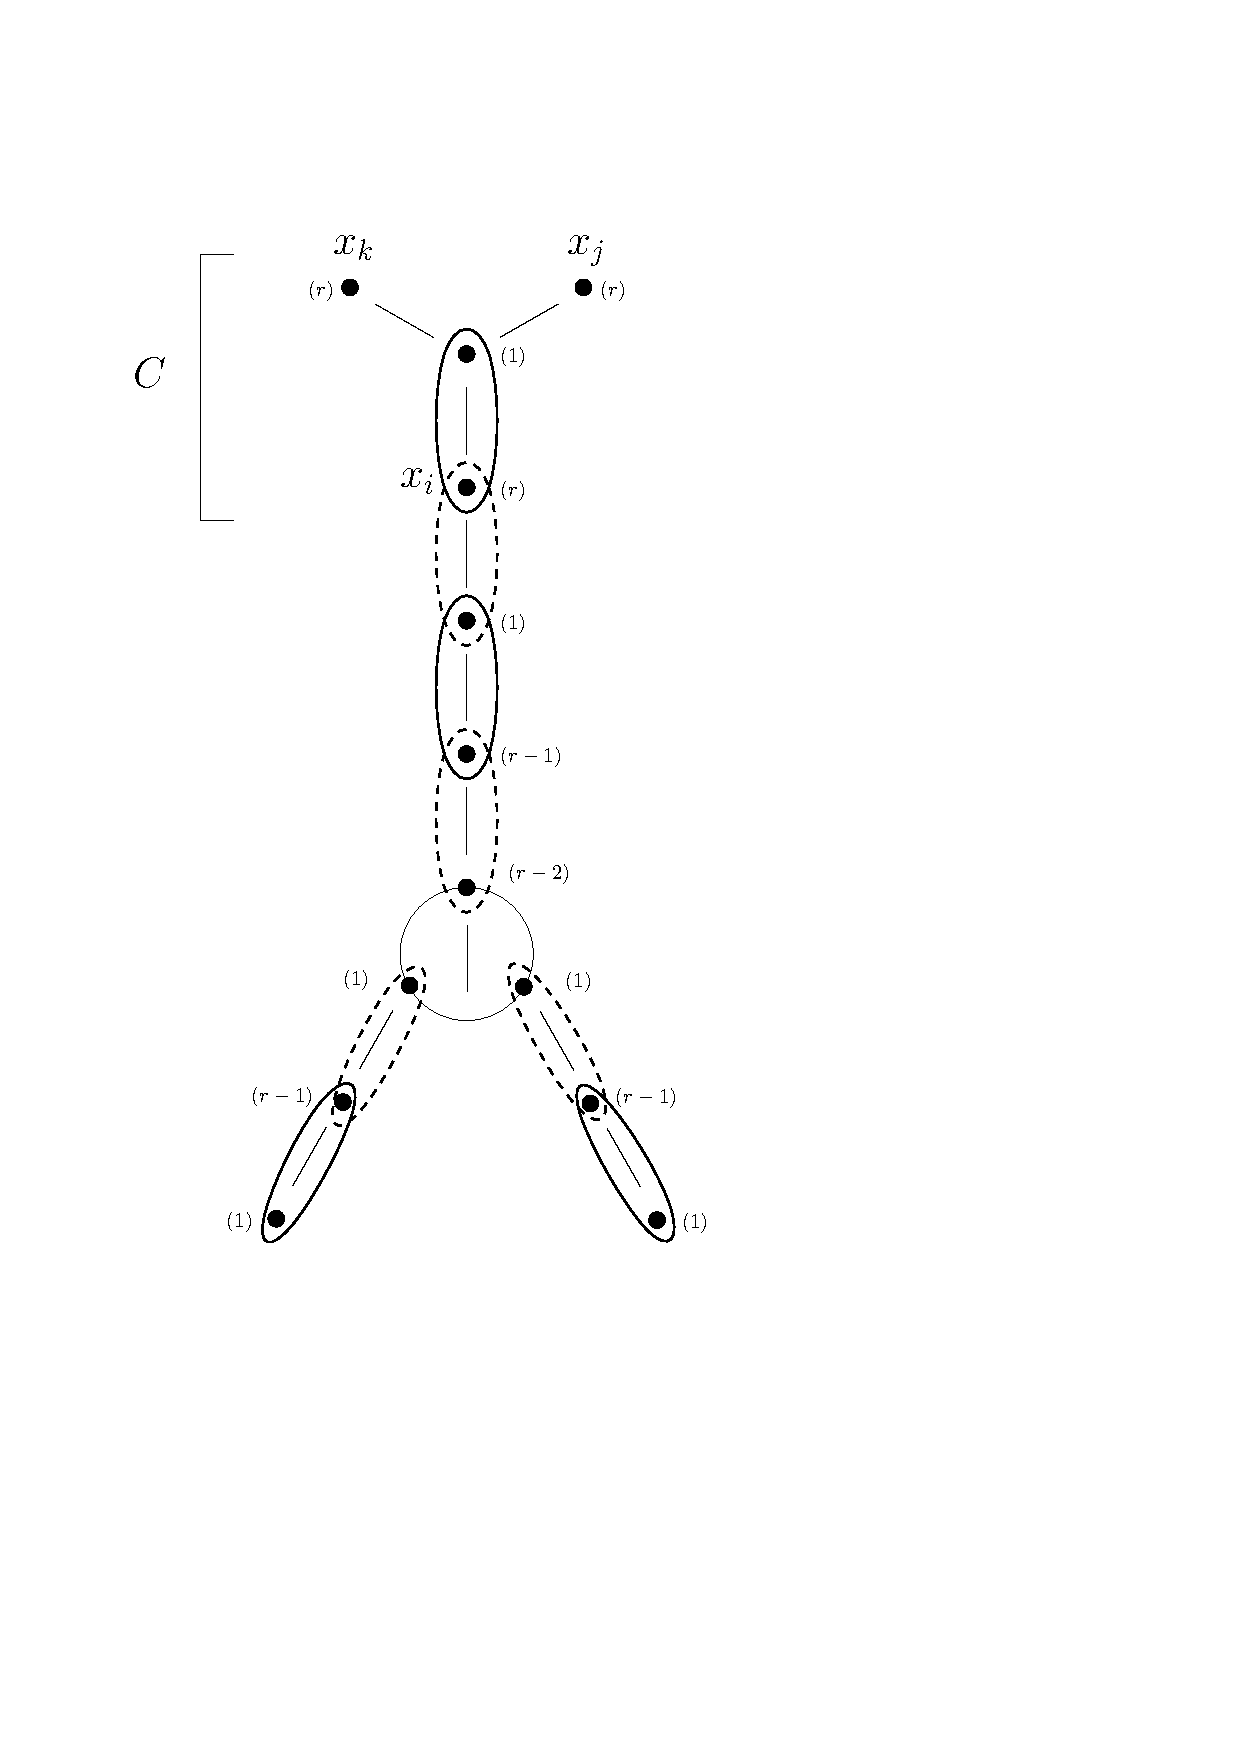
\includegraphics[page=1,width=.33\linewidth]{figs/correctanimloose.pdf}
\end{center}
}

\frame{ \frametitle{Hardness}

We show that:

\begin{itemize}
\item pos SAT $\rightarrow$ instance with OPT=1
\item neg SAT $\rightarrow$ instance with OPT $\ge c$ ~(for some approx factor $c \in [1,2]$)
\end{itemize}
\pause \vskip .35cm


If SAT is neg, how will the instance ``correct itself''?

\begin{itemize}
\item correcting within chain would cost 2
\item correcting at a clause would cost 2 (or would it!)
\end{itemize}
\pause \vskip .35cm

Only other option:
\begin{itemize}
\item correcting at a splitter
\end{itemize}
}



\frame{ \frametitle{Hardness}


\begin{center}
  \includegraphics<1>[page=1,width=.33\linewidth]{figs/correctanimloose.pdf}
\pause
  \includegraphics<2>[page=1,width=.33\linewidth]{figs/correctanim.pdf}
%  \only<1>{\\Obs: both directions can't be bad---consider $\deg_L(v)$ v. $\deg_R(v)$.}
\pause
  \includegraphics<3>[page=2,width=.33\linewidth]{figs/correctanim.pdf}
%  \only<2>{\\Obs: If $\deg_L(v) \le \deg_R(v)$, still true after moving left.}
\pause
  \includegraphics<4>[page=1,width=.33\linewidth]{figs/correctanim.pdf}
\pause
  \includegraphics<5>[page=3,width=.33\linewidth]{figs/correctanim.pdf}
\pause
  \includegraphics<6>[page=1,width=.33\linewidth]{figs/correctanim.pdf}
\pause
  \includegraphics<7>[page=4,width=.33\linewidth]{figs/correctanim.pdf}
\pause
  \includegraphics<8>[page=5,width=.33\linewidth]{figs/correctanim.pdf}
\pause
  \includegraphics<9>[page=6,width=.33\linewidth]{figs/correctanim.pdf}
\pause
  \includegraphics<10>[page=1,width=.33\linewidth]{figs/correctanim.pdf}
\pause
  \includegraphics<11>[page=7,width=.33\linewidth]{figs/correctanim.pdf}
\pause
  \includegraphics<12>[page=8,width=.33\linewidth]{figs/correctanim.pdf}
\pause
  \includegraphics<13>[page=9,width=.33\linewidth]{figs/correctanim.pdf}
\end{center}
}


%\frame{ \frametitle{Hardness}
%
%%\begin{center}
%%  \includegraphics<1>[width=.75\linewidth]{hardness0.png}
%%\pause
%%  \includegraphics<2>[width=.75\linewidth]{hardness1.png}
%%\pause
%%  \includegraphics<3>[width=.75\linewidth]{hardness2.png}
%%  \only<3>{\\ $\overline{CR}(G') \approx $~cut size$(G) \cdot n^3$}
%%\end{center}
%\begin{center}
%%  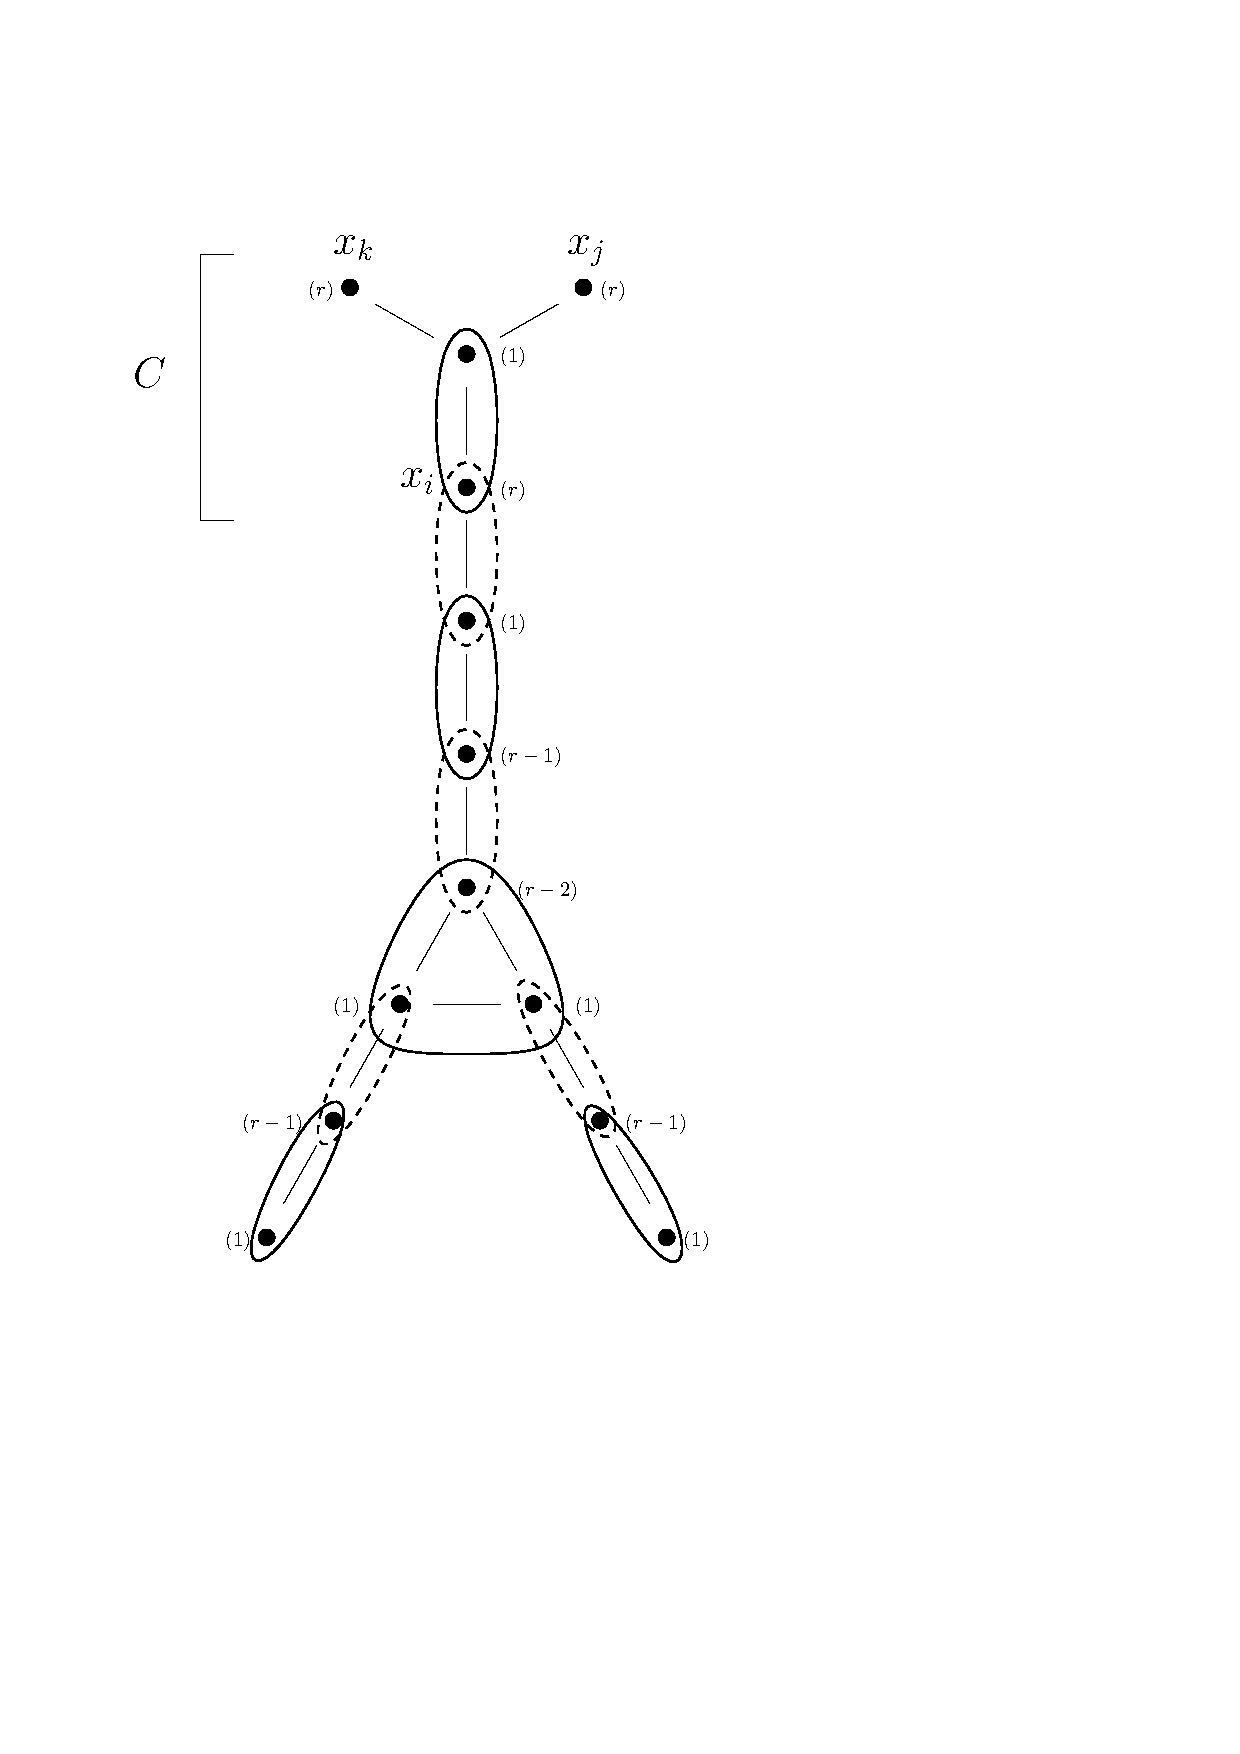
\includegraphics[width=.25\linewidth]{figs/hardness.pdf}
%%\pause
%%  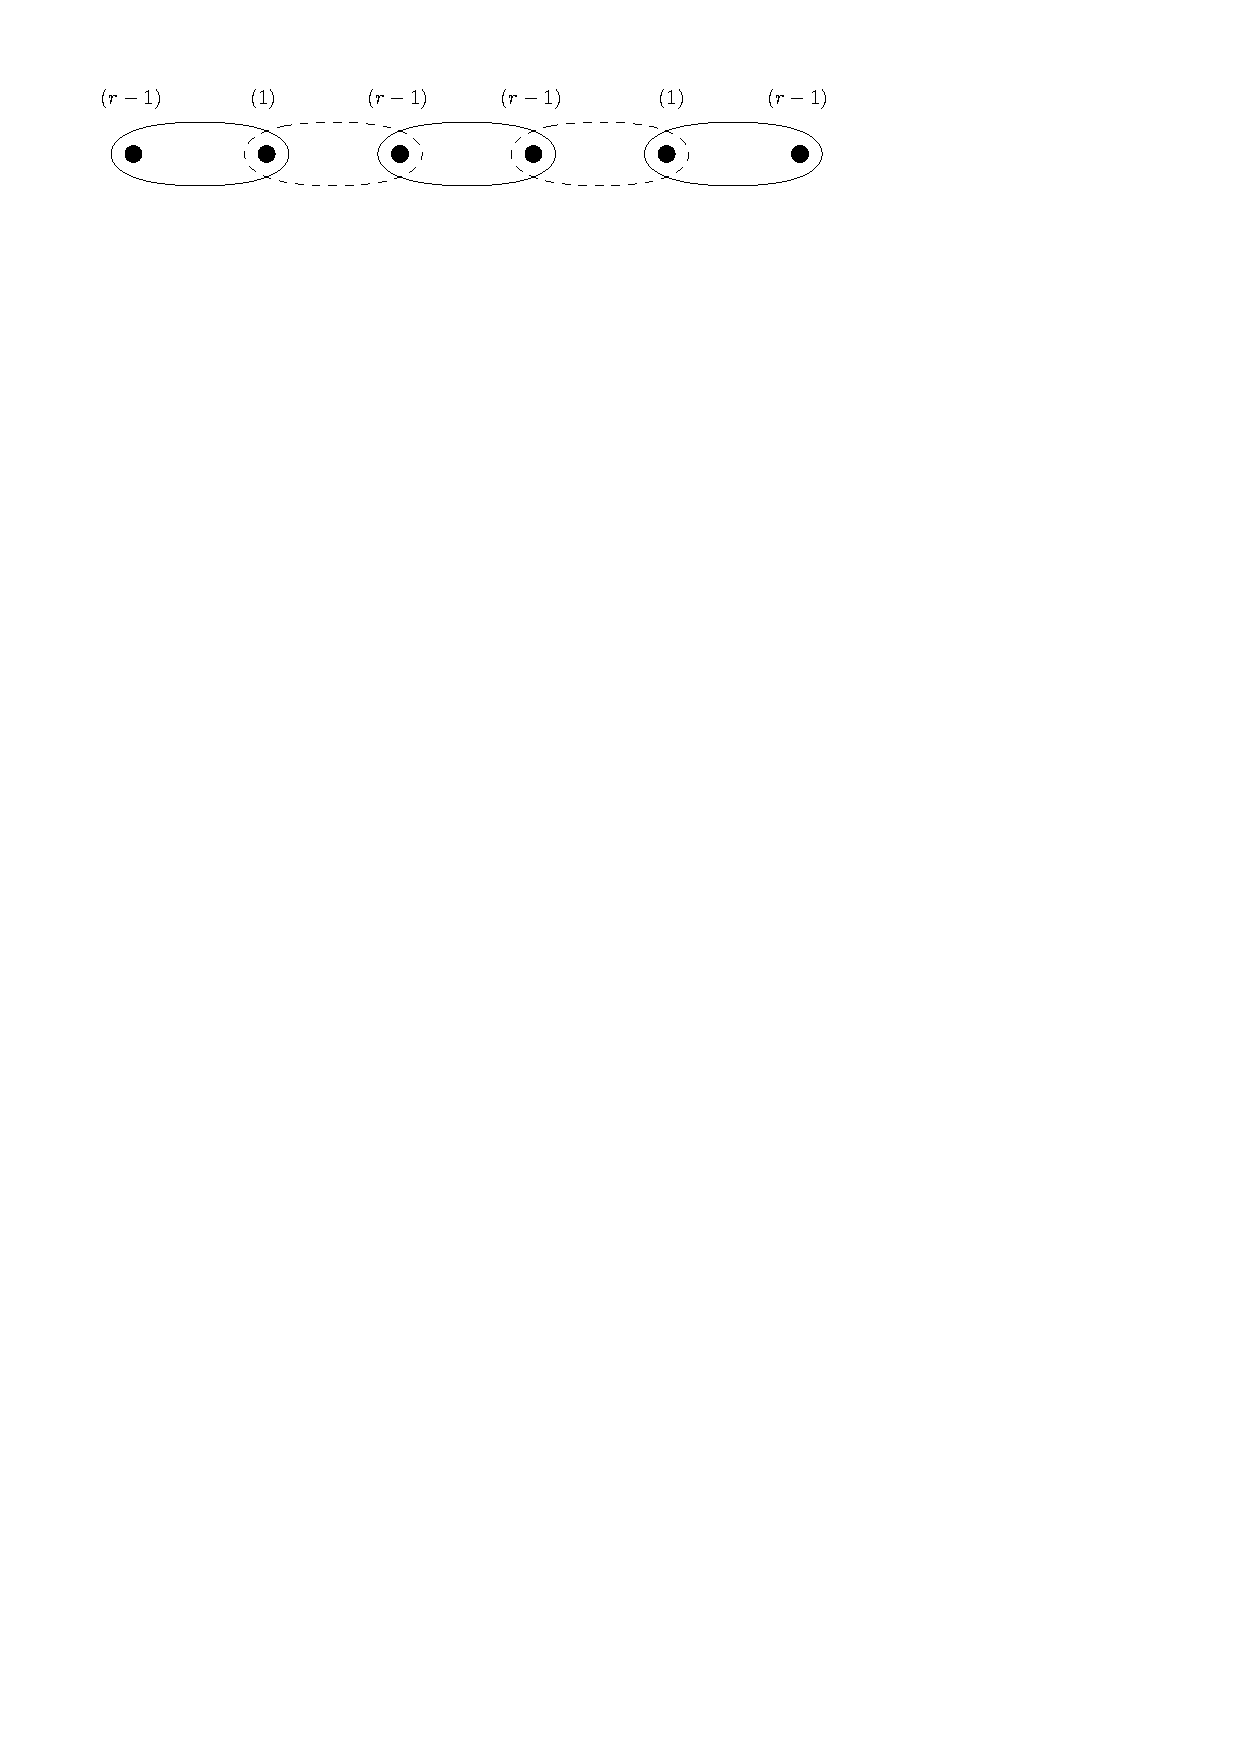
\includegraphics[width=.75\linewidth]{figs/negation.pdf}
%%\pause
%  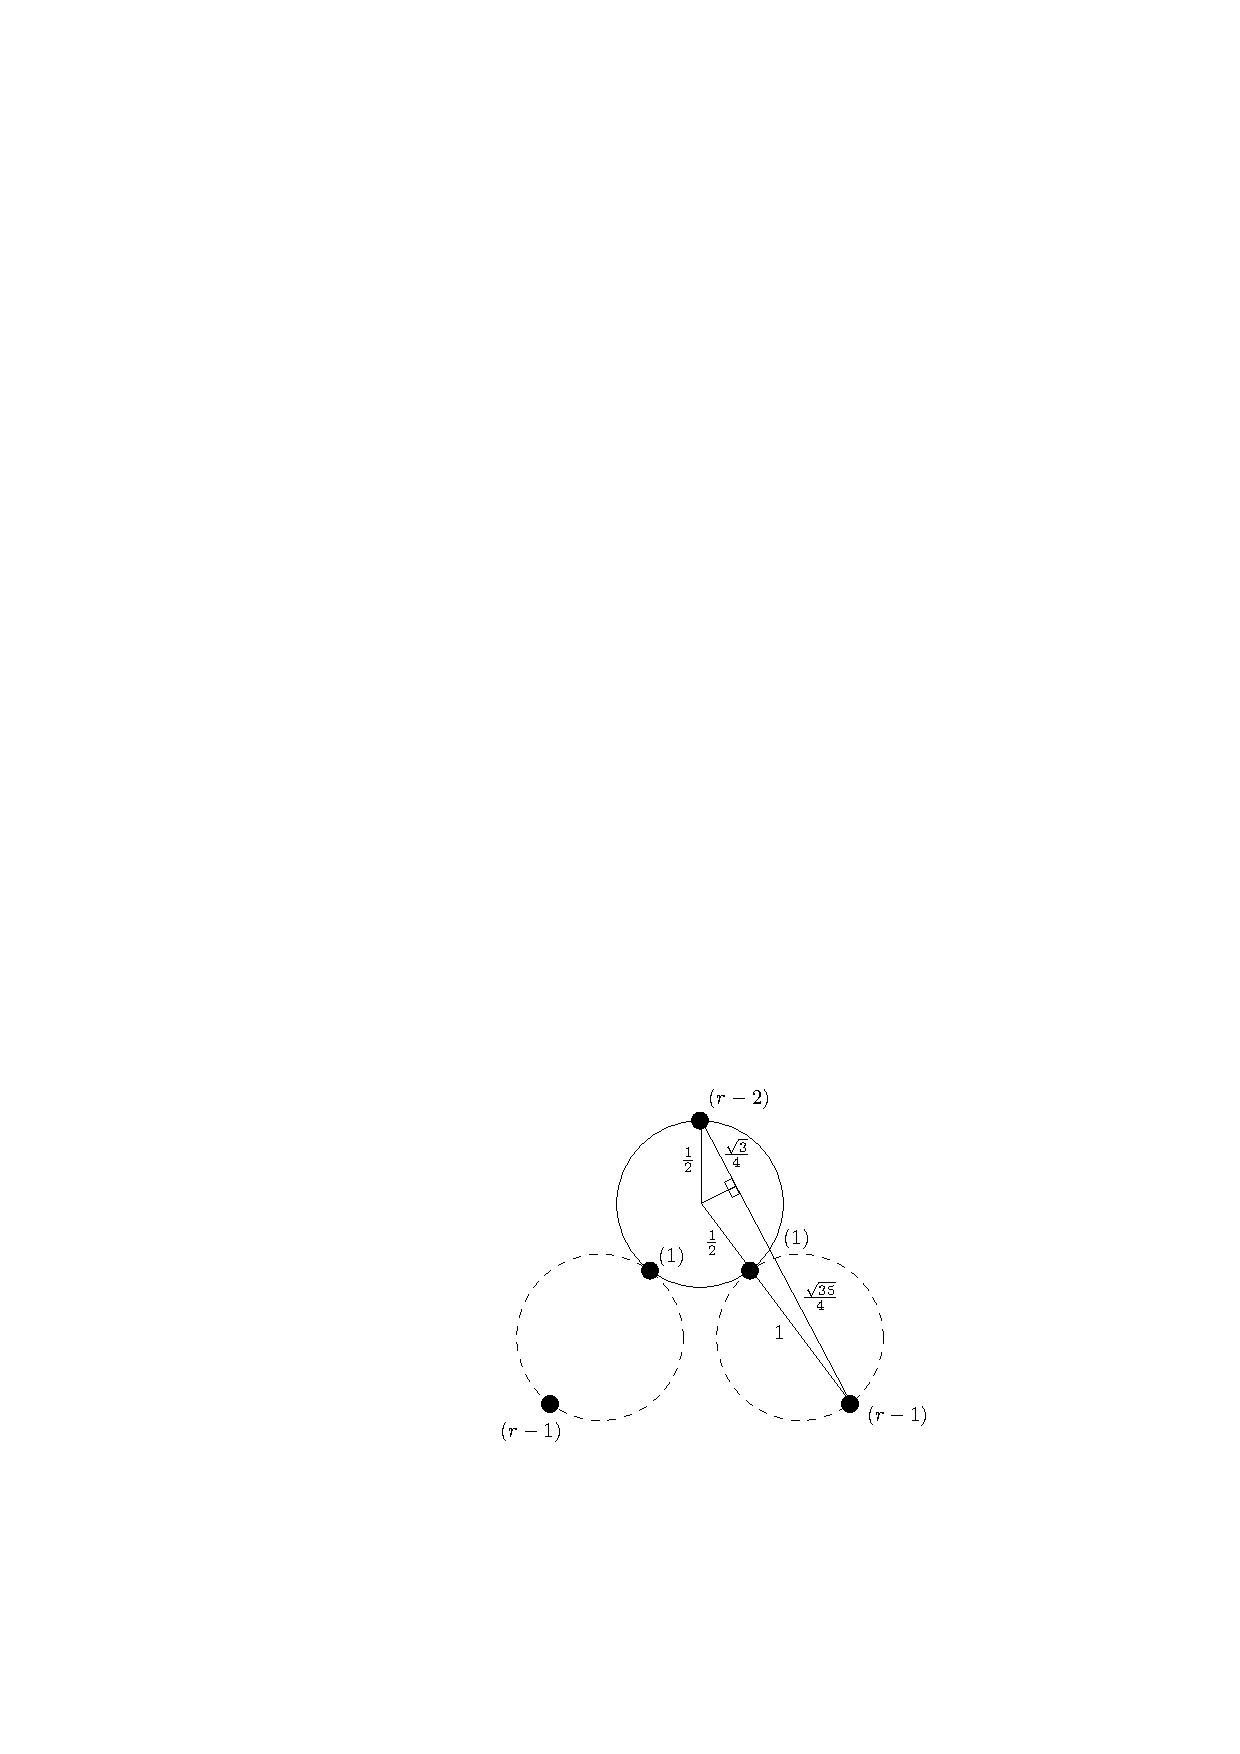
\includegraphics[width=.335\linewidth]{figs/splitter.pdf}
%%\pause
%%  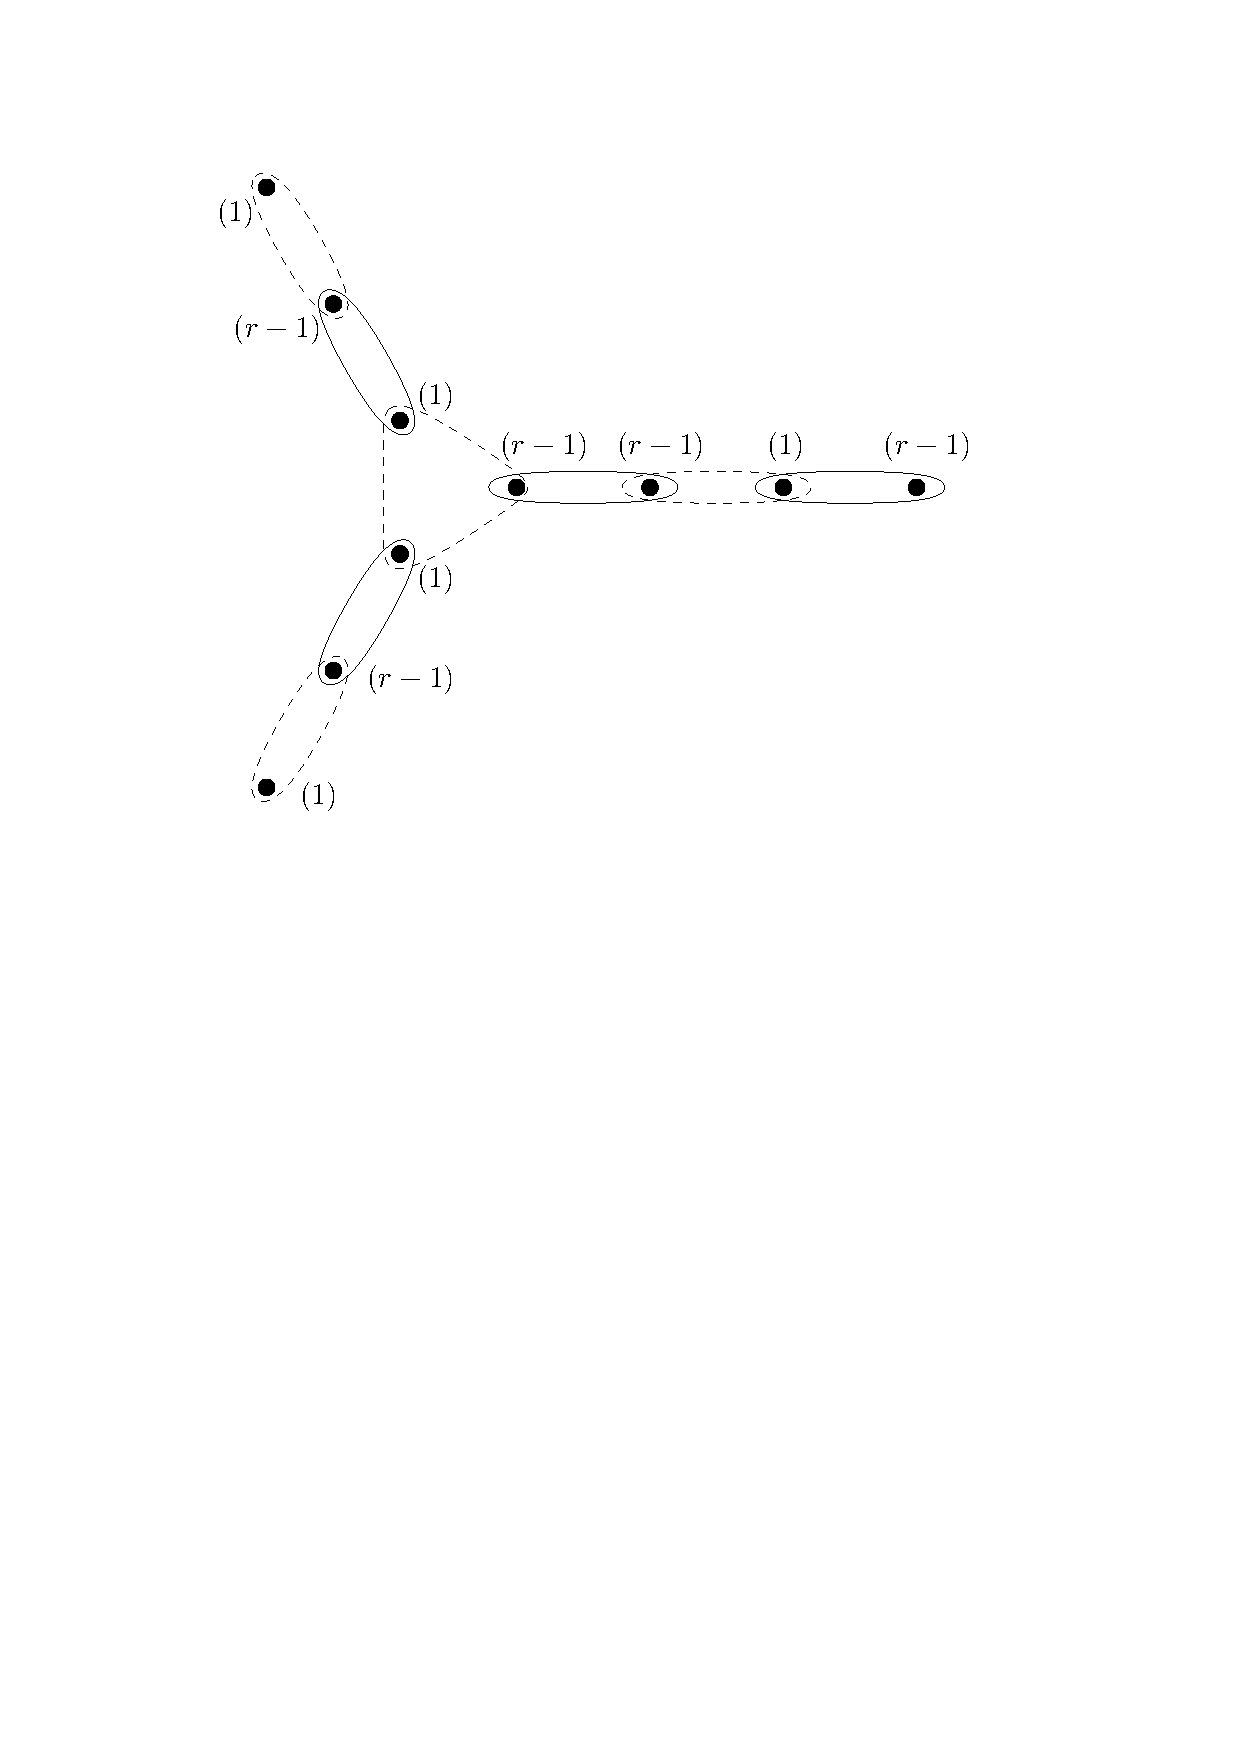
\includegraphics[width=.75\linewidth]{figs/nandgadget.pdf}
%\end{center}
%}

%\frame{ \frametitle{Hardness}
%
%%\begin{center}
%%  \includegraphics<1>[width=.75\linewidth]{hardness0.png}
%%\pause
%%  \includegraphics<2>[width=.75\linewidth]{hardness1.png}
%%\pause
%%  \includegraphics<3>[width=.75\linewidth]{hardness2.png}
%%  \only<3>{\\ $\overline{CR}(G') \approx $~cut size$(G) \cdot n^3$}
%%\end{center}
%\begin{center}
%  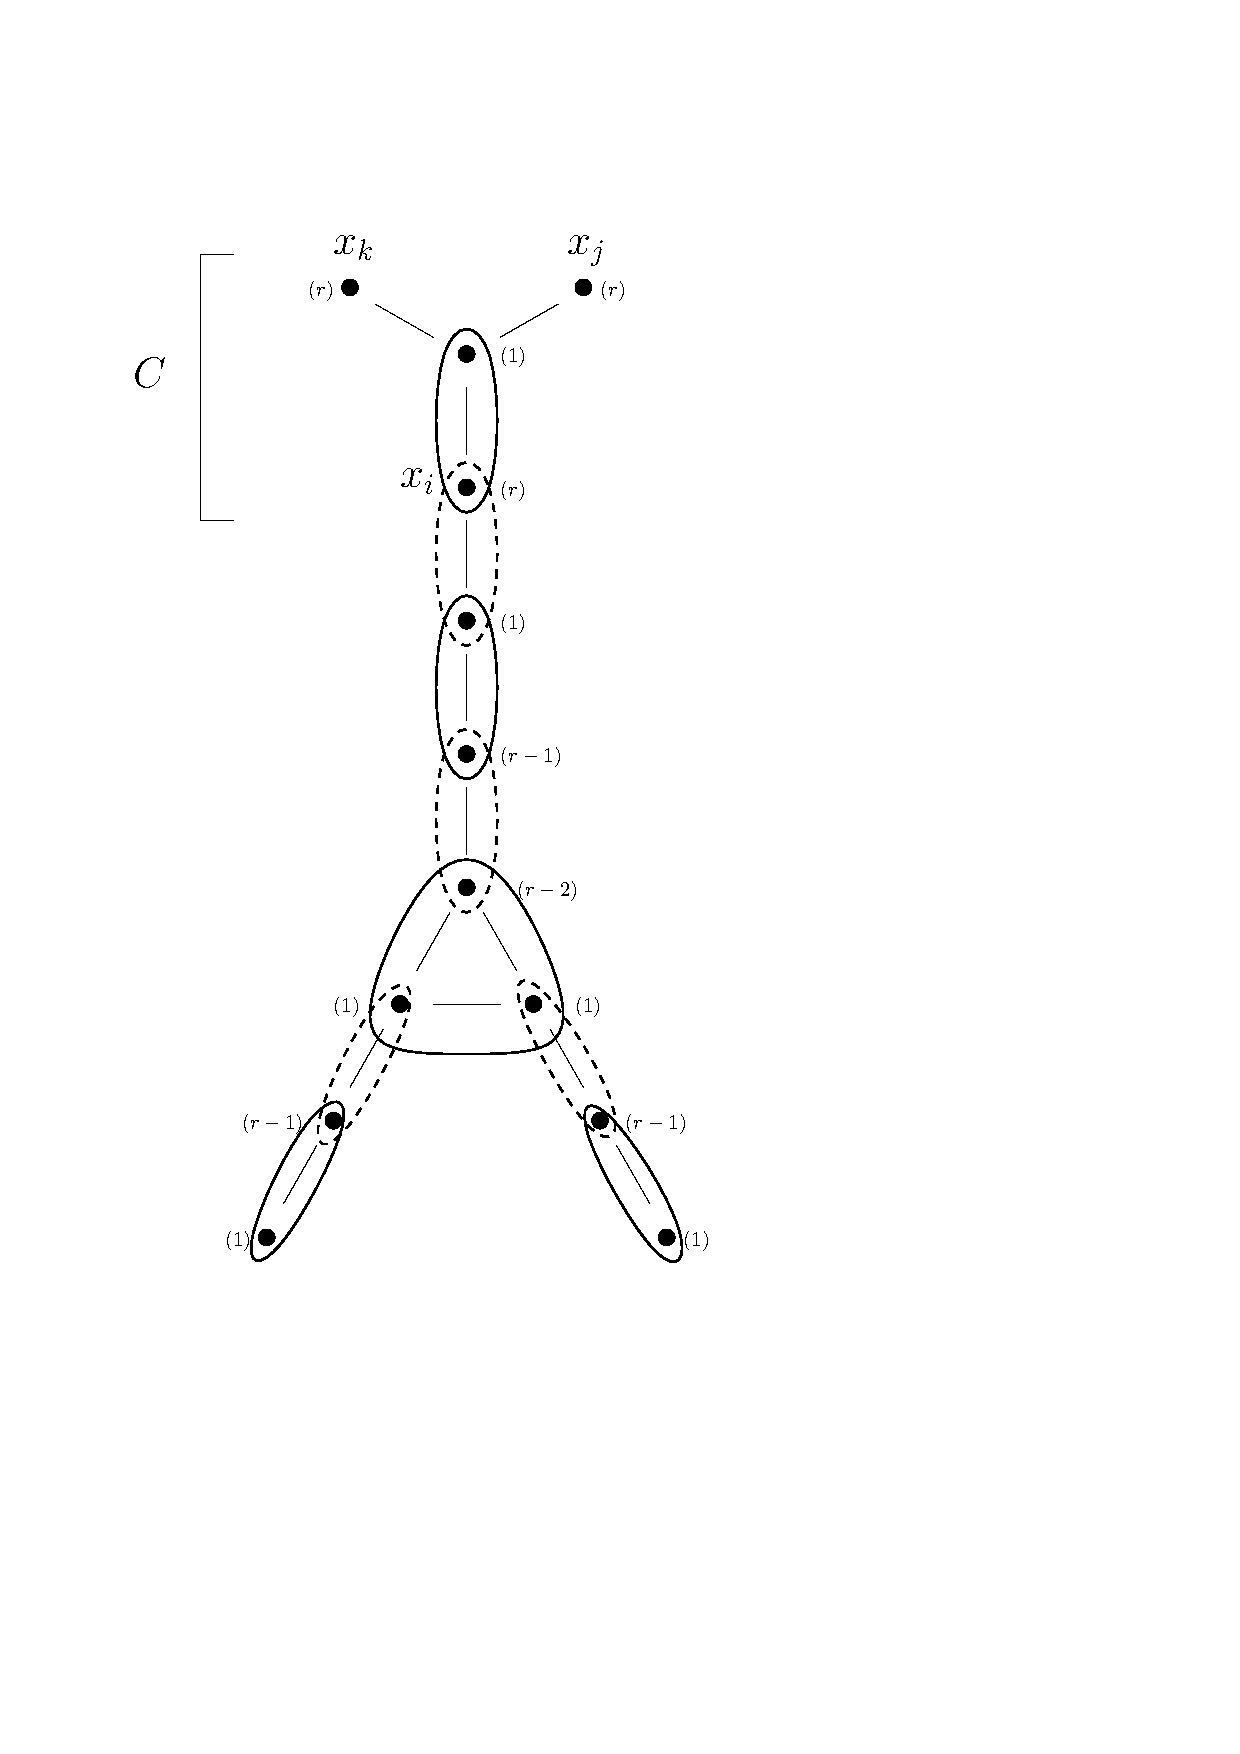
\includegraphics[width=.25\linewidth]{figs/hardness.pdf}
%\pause
%  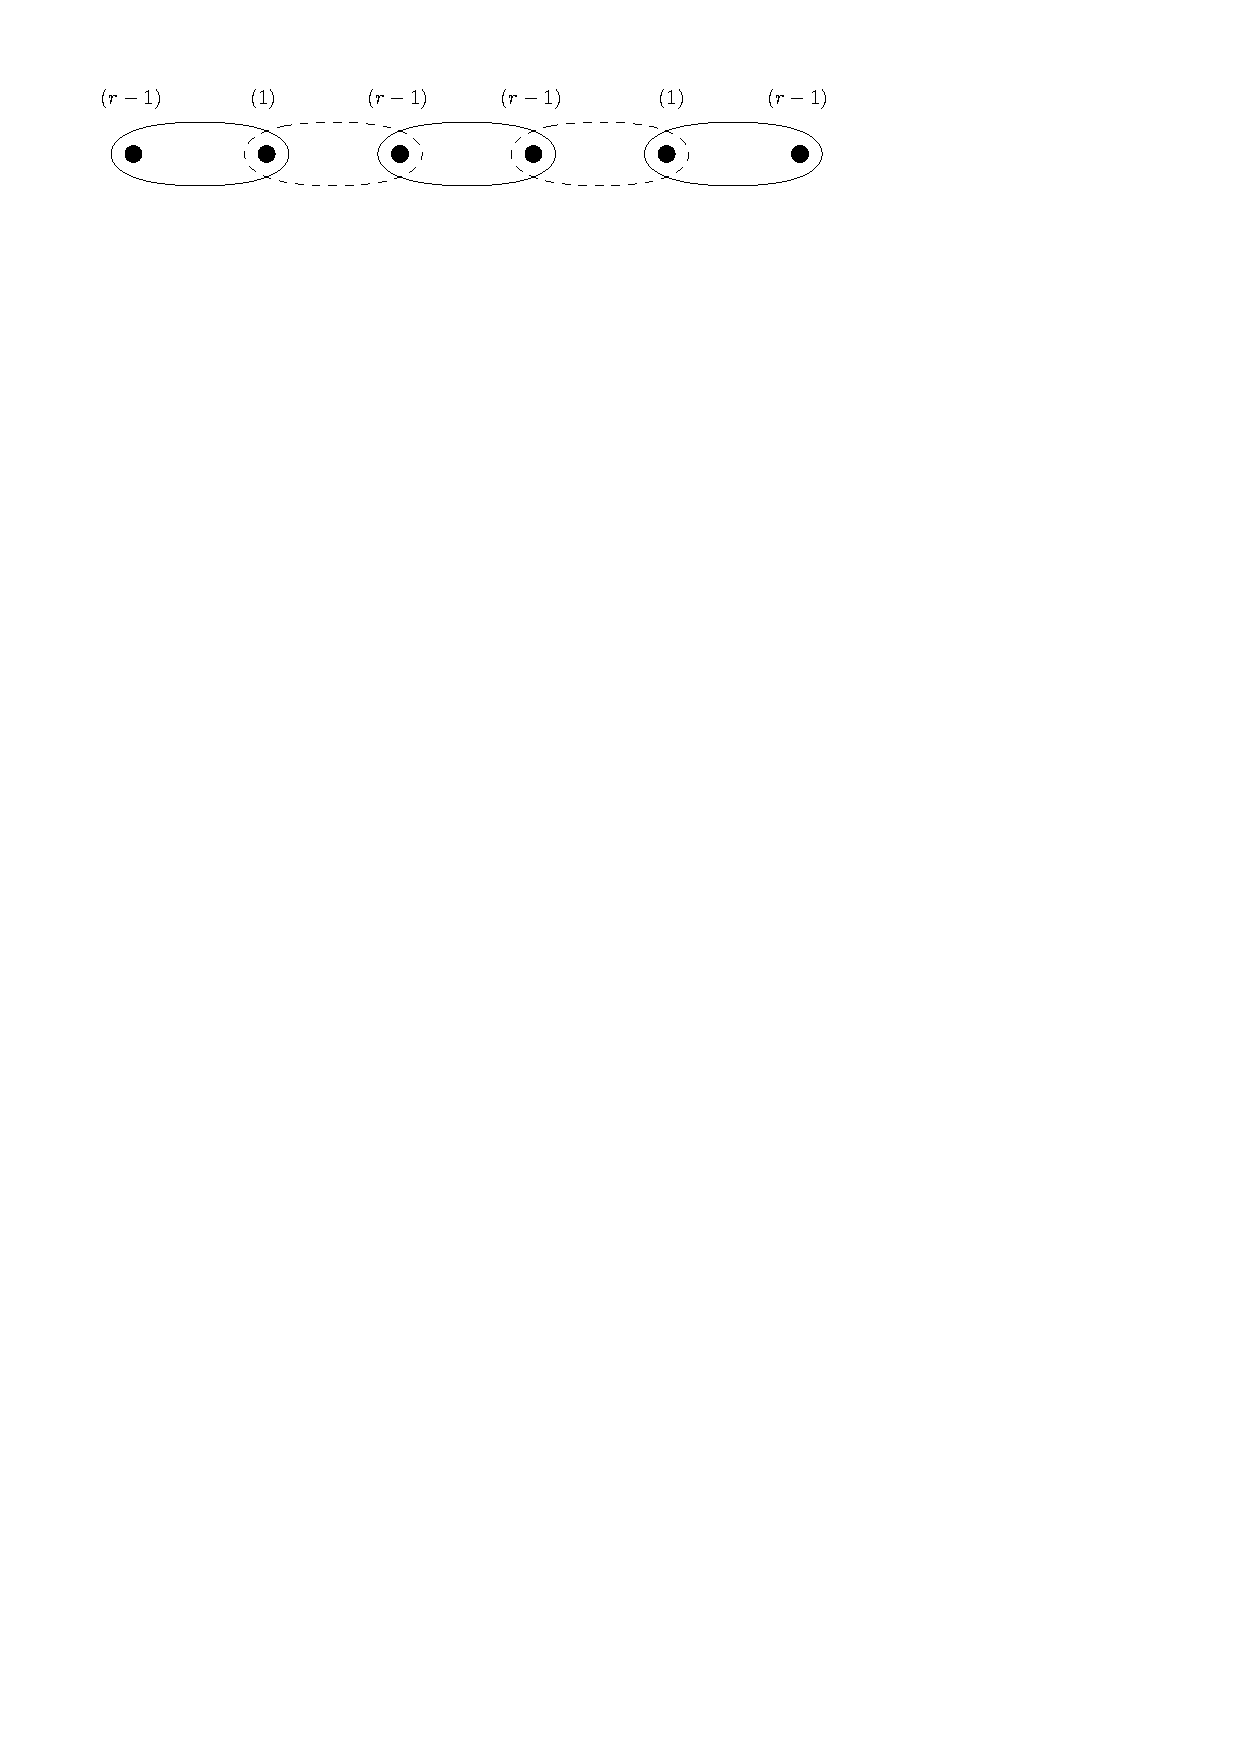
\includegraphics[width=.75\linewidth]{figs/negation.pdf}
%\pause
%  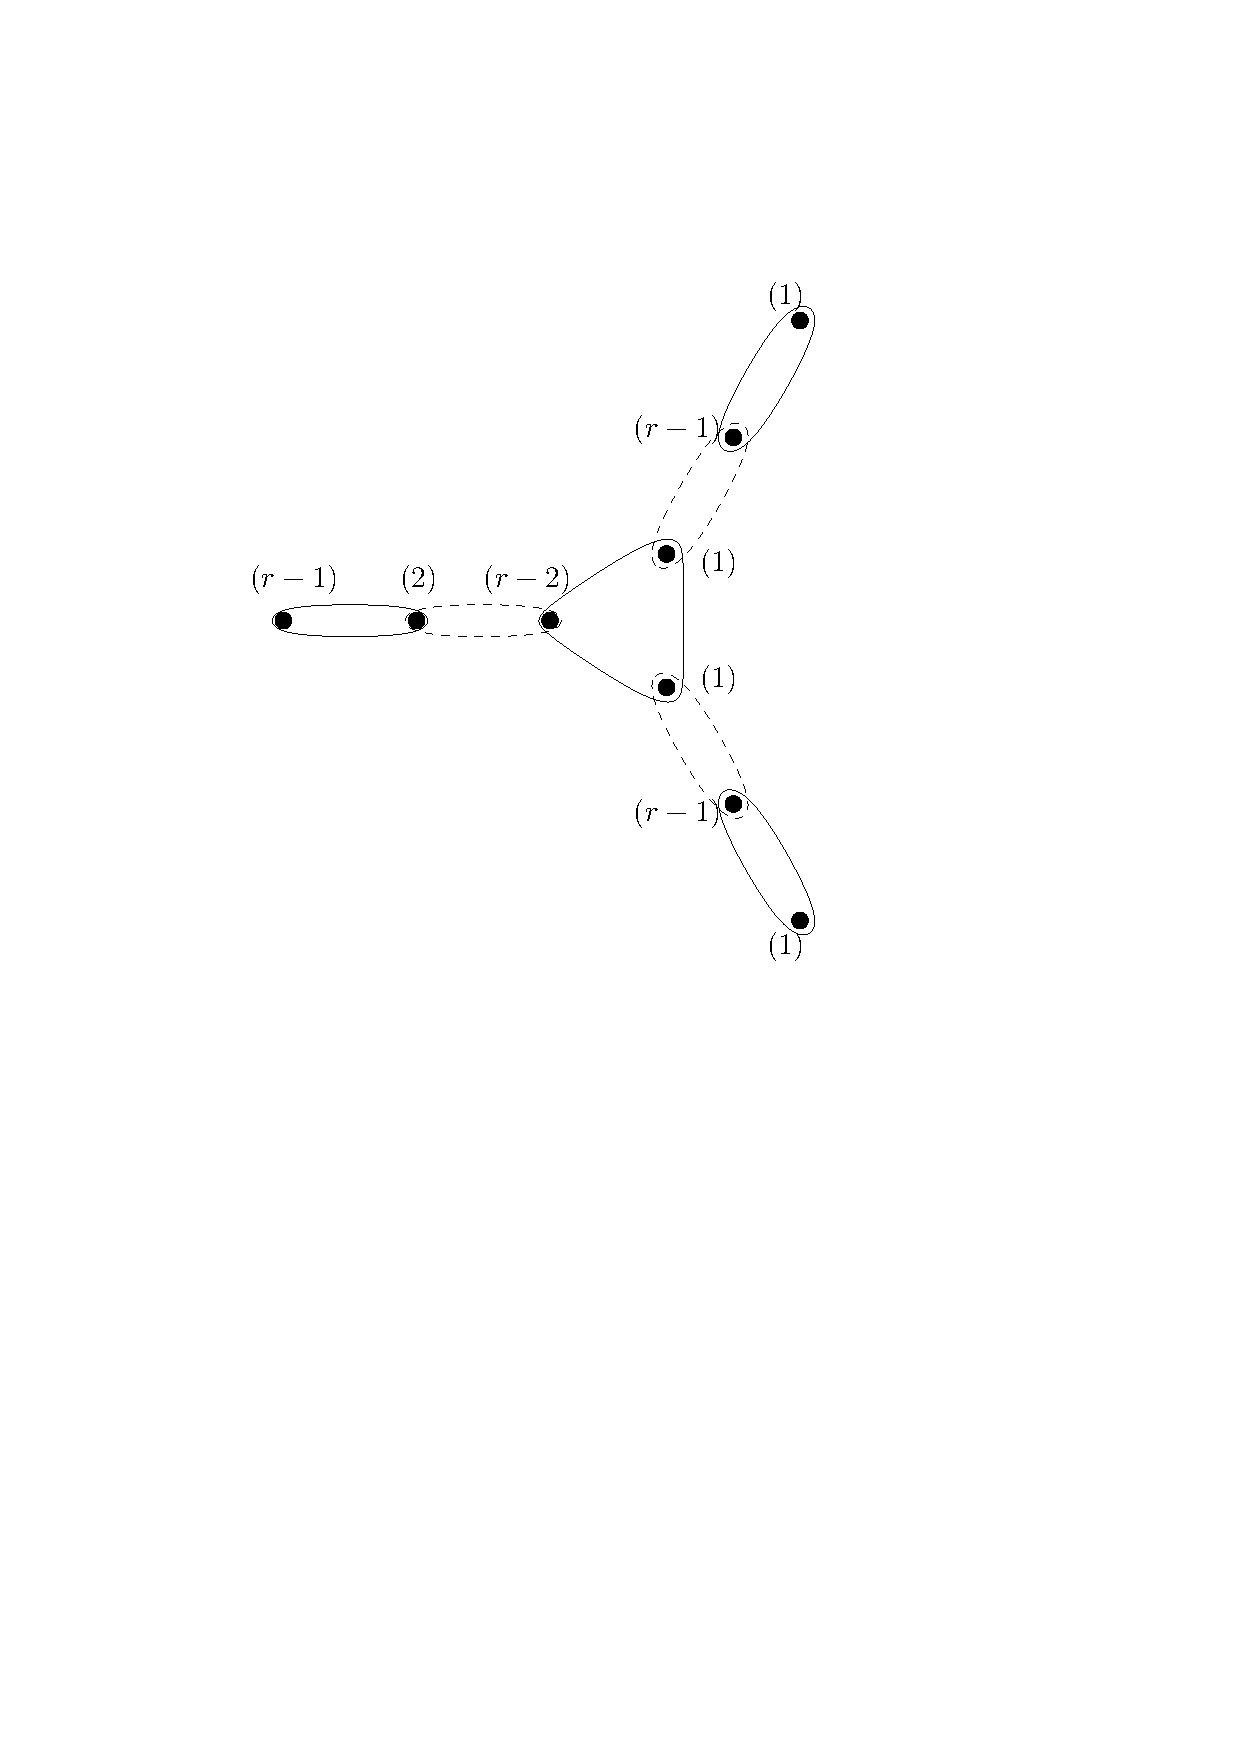
\includegraphics[width=.75\linewidth]{figs/splittergadget.pdf}
%\pause
%  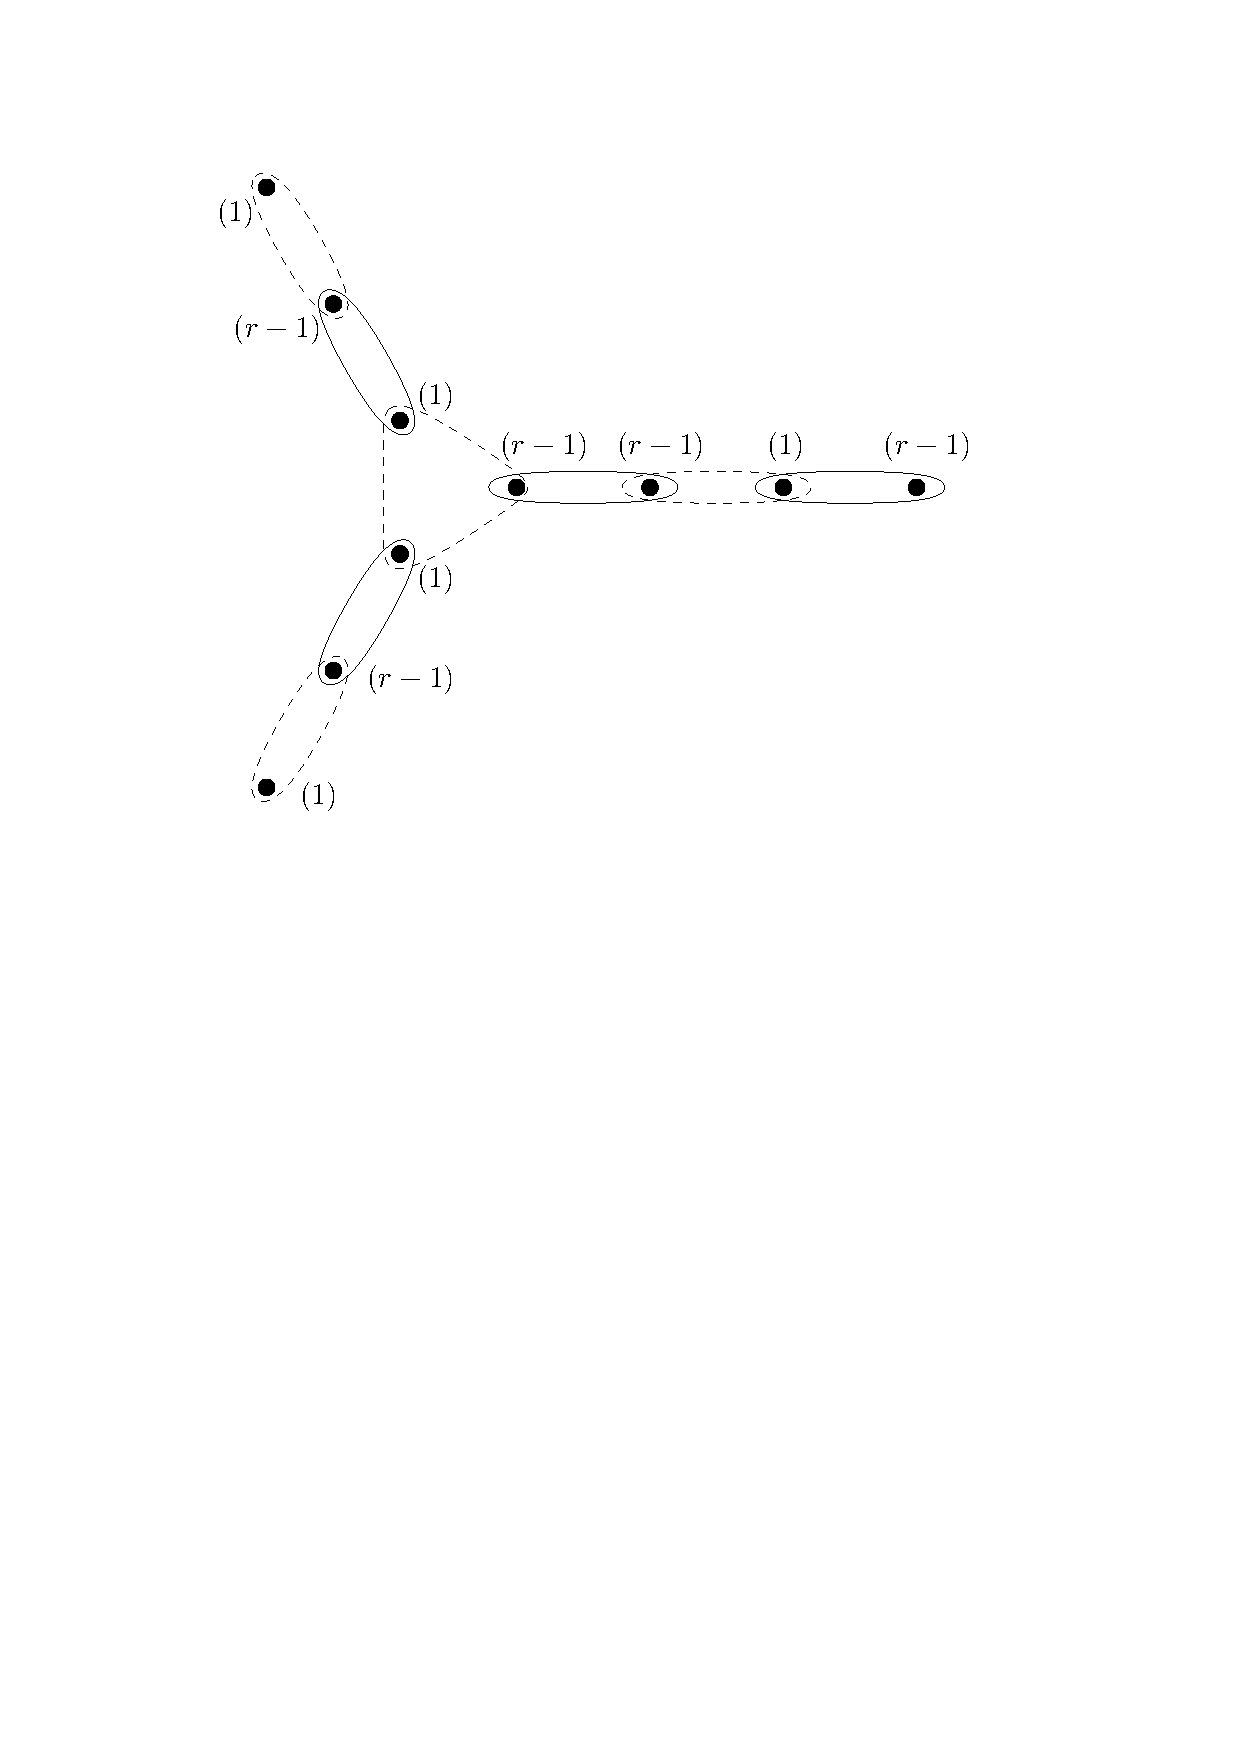
\includegraphics[width=.75\linewidth]{figs/nandgadget.pdf}
%\end{center}
%}

%\frame{ \frametitle{Hardness}
%
%%\begin{center}
%%  \includegraphics<1>[width=.75\linewidth]{hardness0.png}
%%\pause
%%  \includegraphics<2>[width=.75\linewidth]{hardness1.png}
%%\pause
%%  \includegraphics<3>[width=.75\linewidth]{hardness2.png}
%%  \only<3>{\\ $\overline{CR}(G') \approx $~cut size$(G) \cdot n^3$}
%%\end{center}
%\begin{center}
%  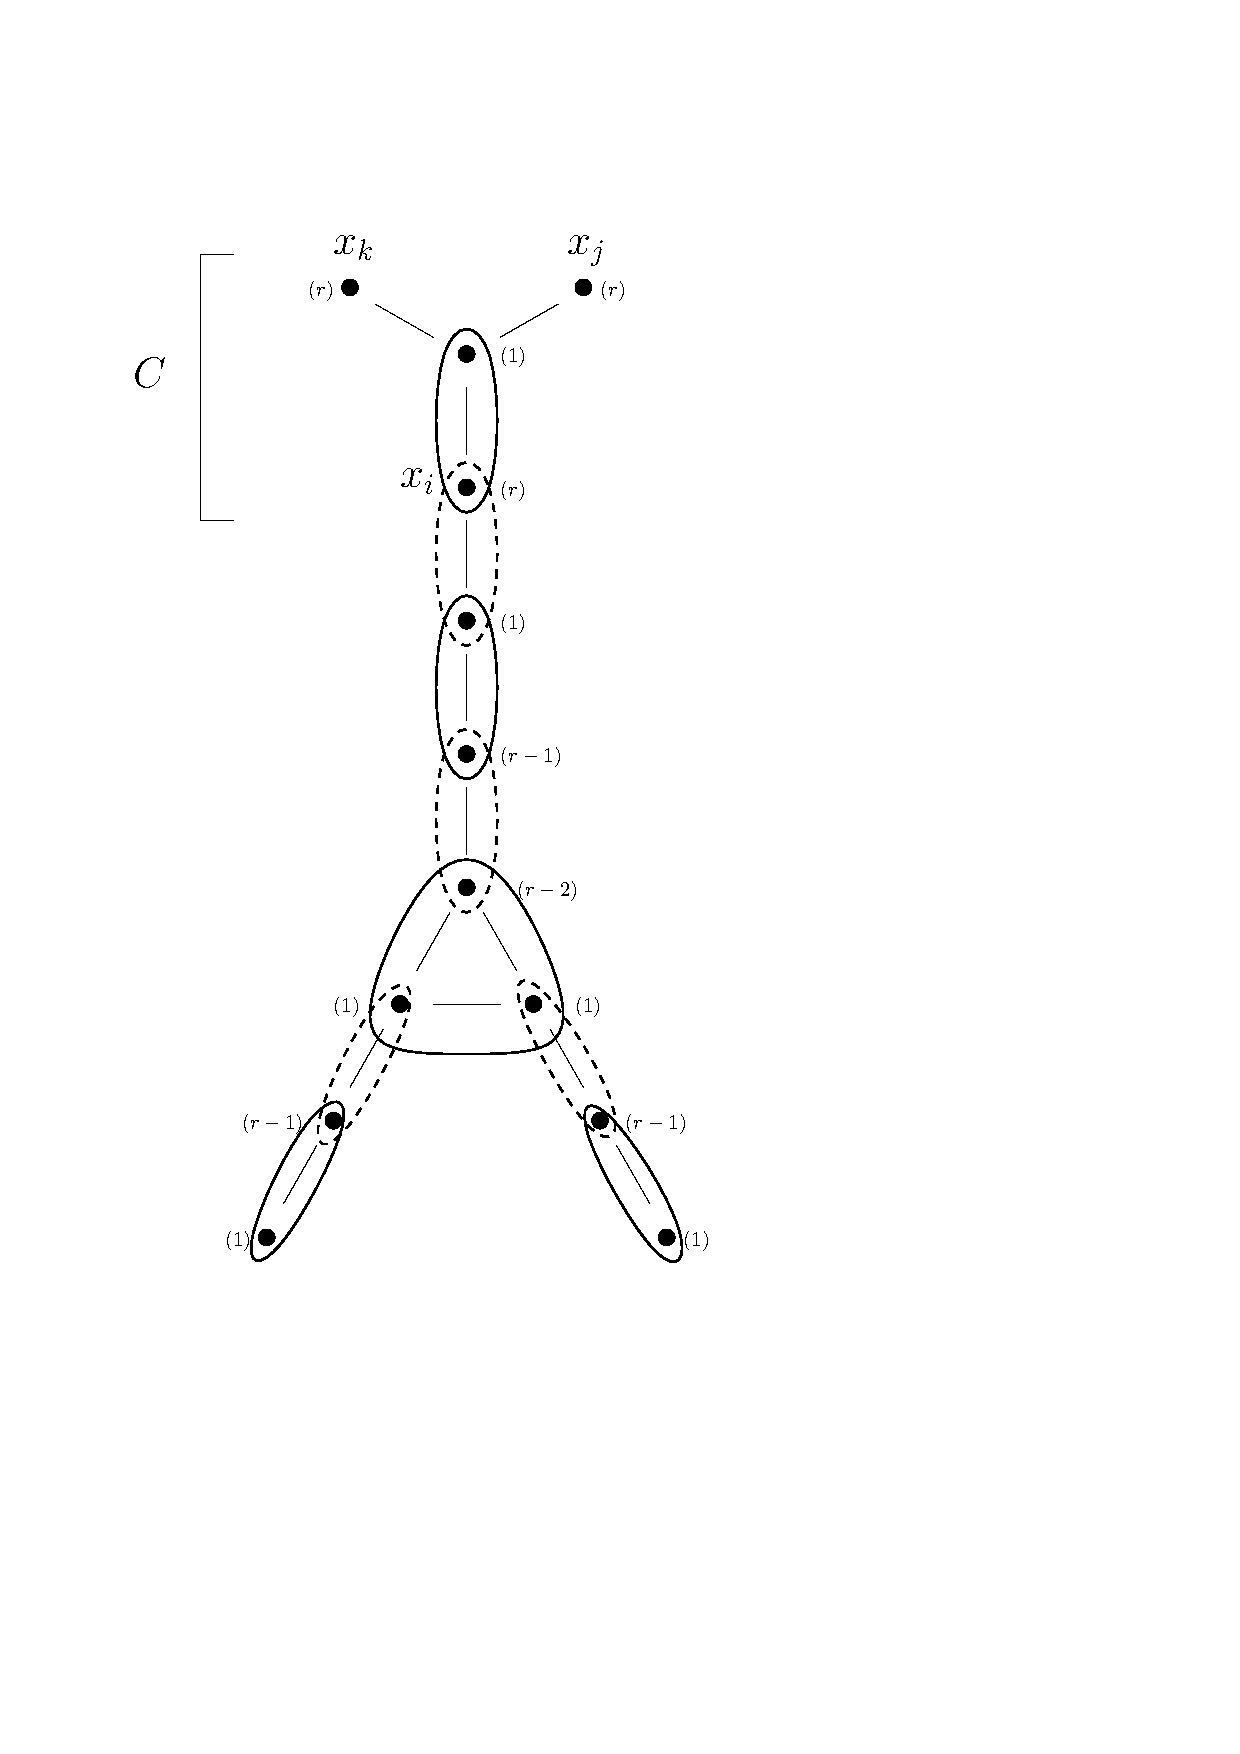
\includegraphics[width=.25\linewidth]{figs/hardness.pdf}
%\pause
%  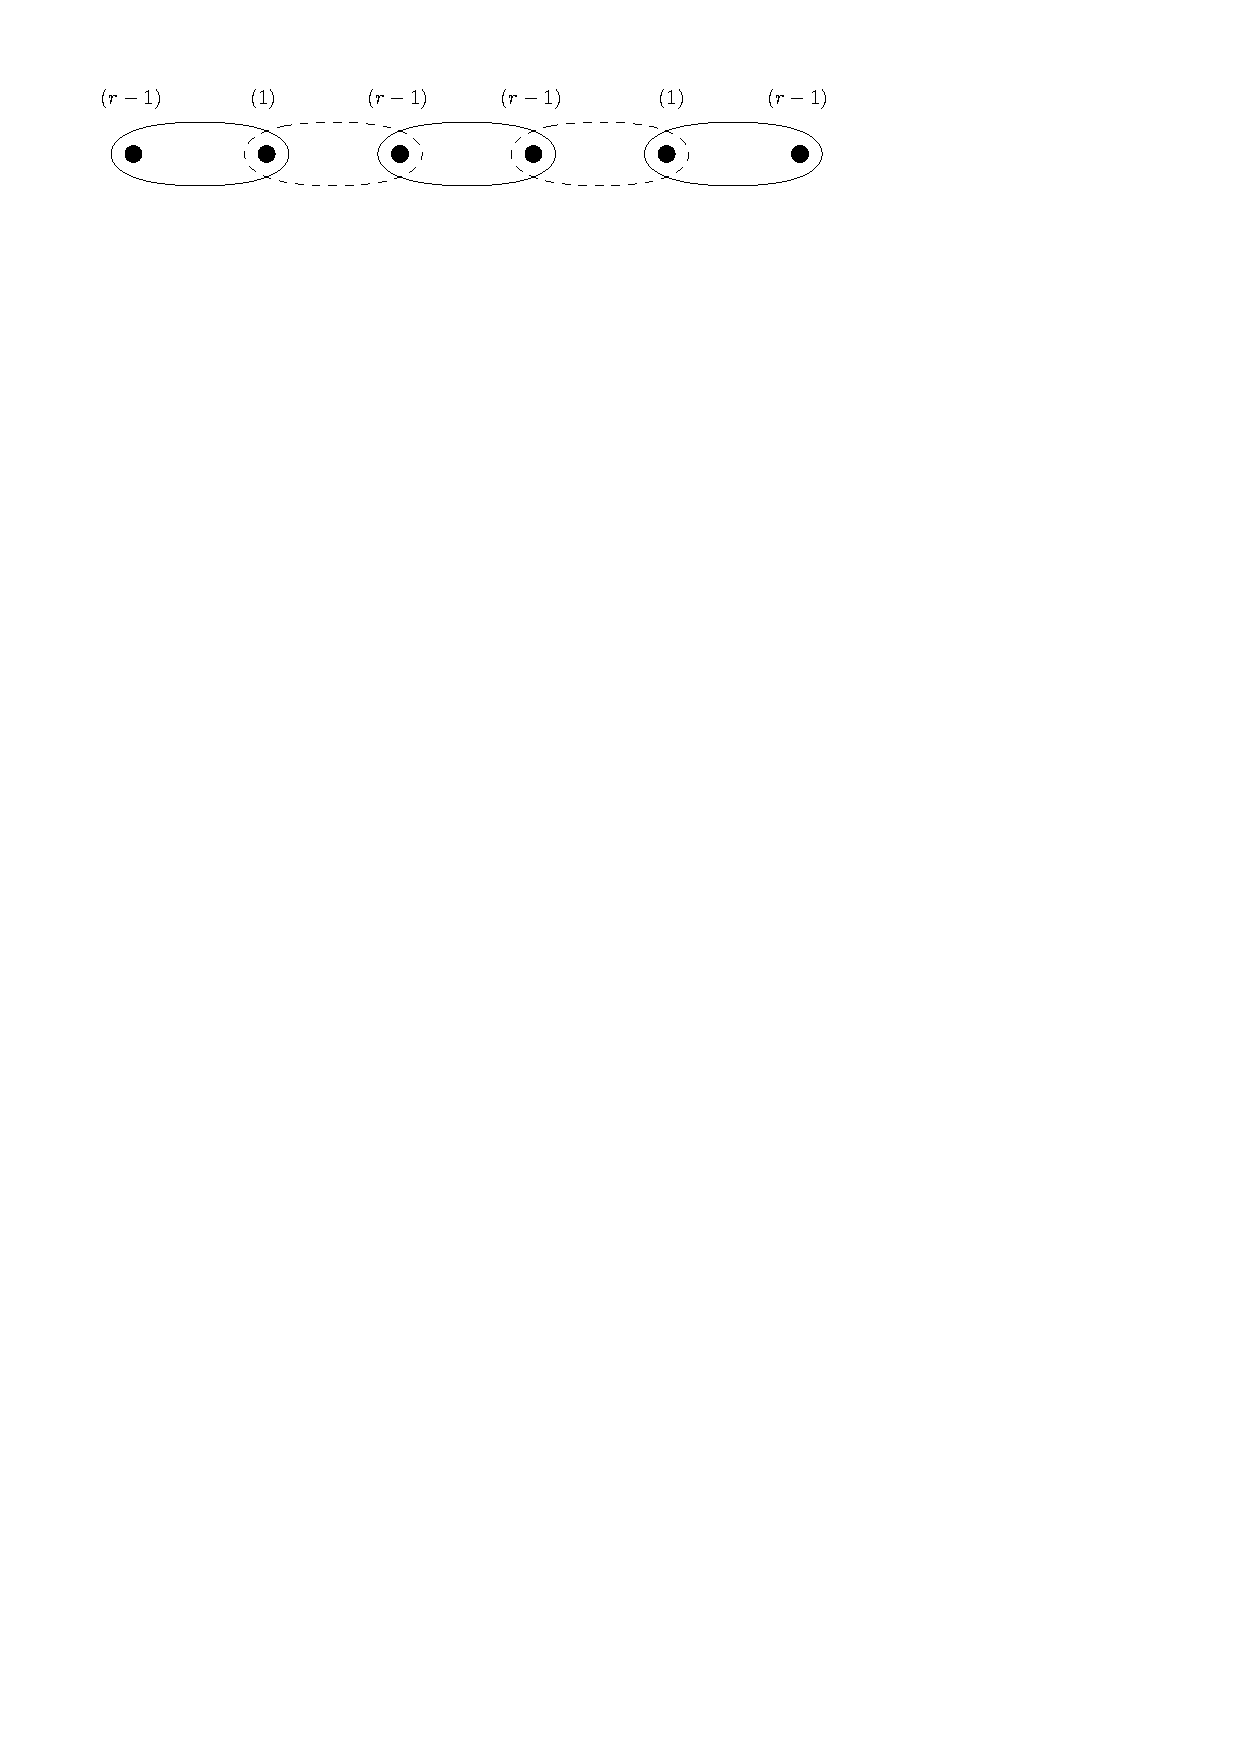
\includegraphics[width=.75\linewidth]{figs/negation.pdf}
%\pause
%  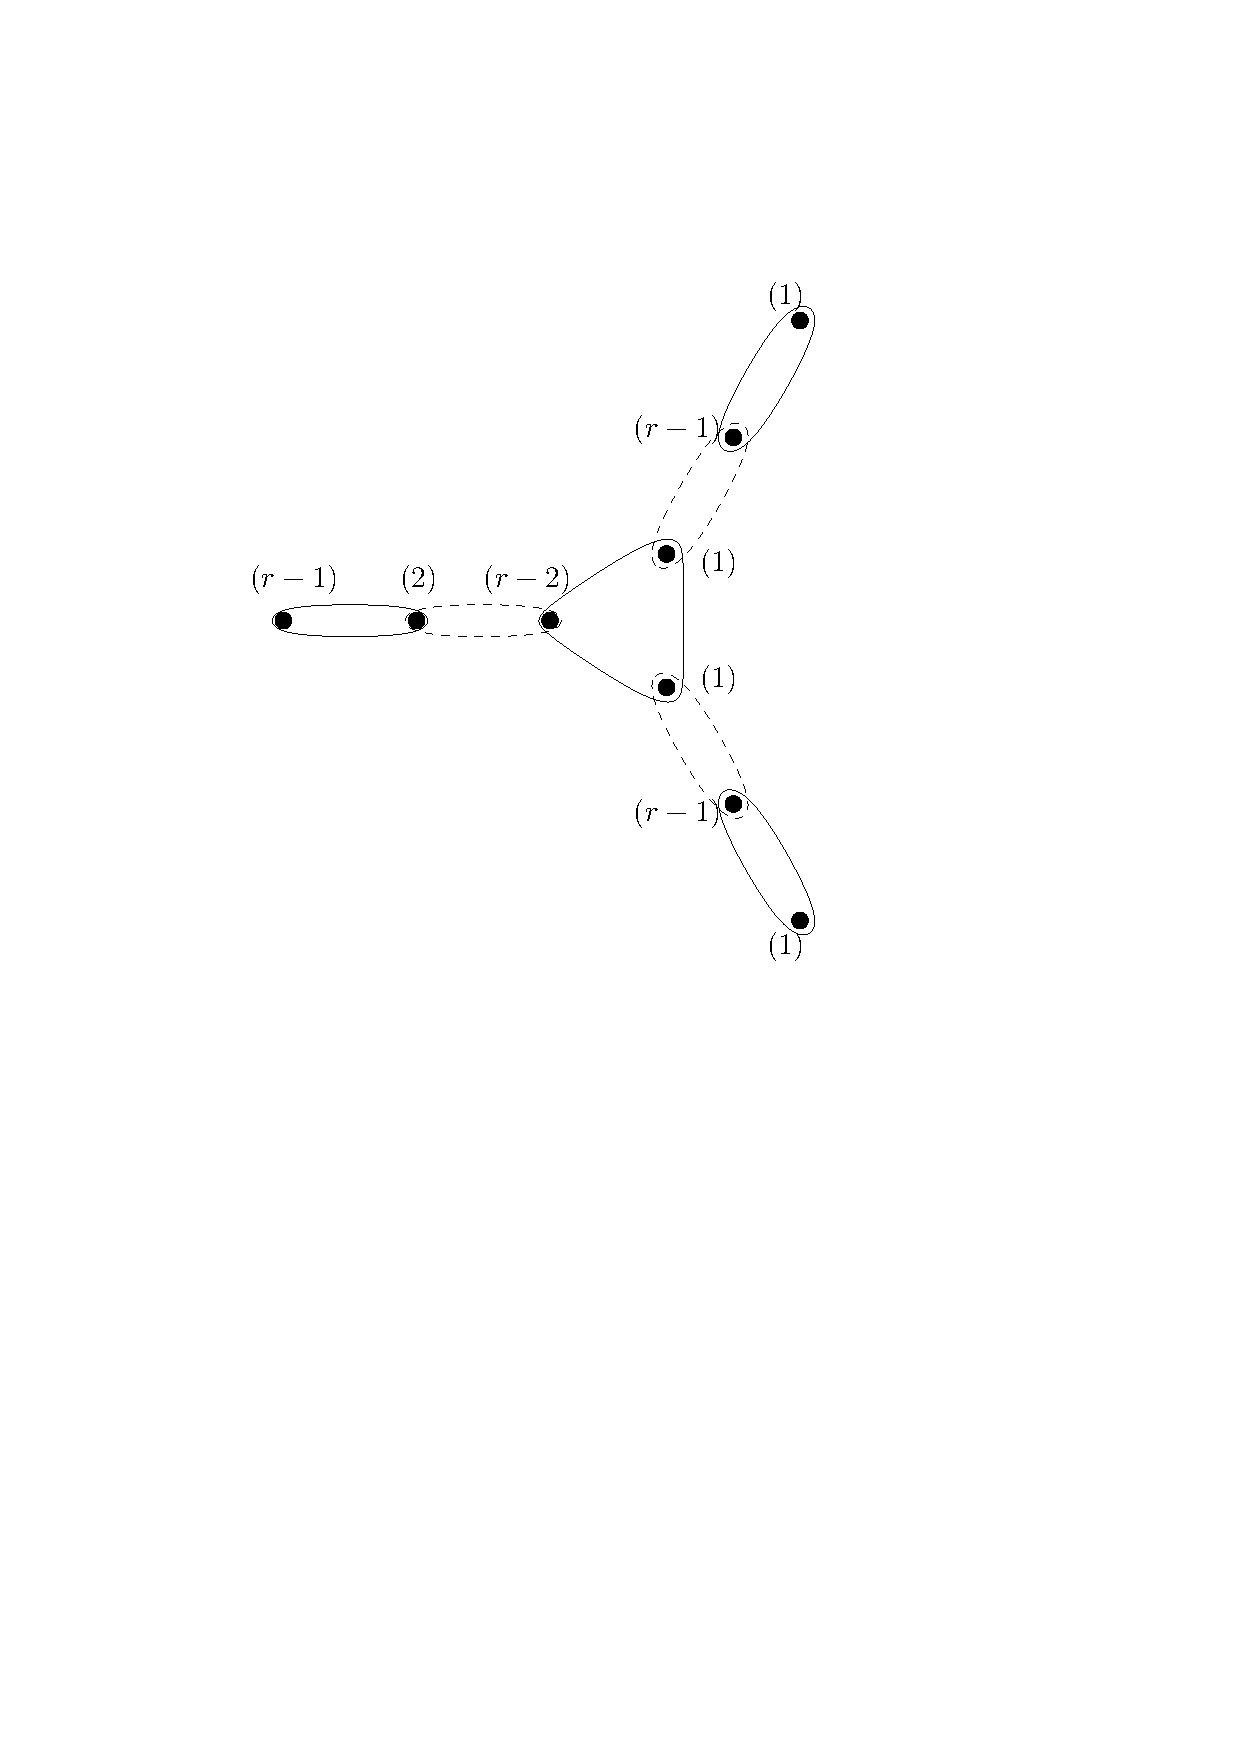
\includegraphics[width=.75\linewidth]{figs/splittergadget.pdf}
%\pause
%  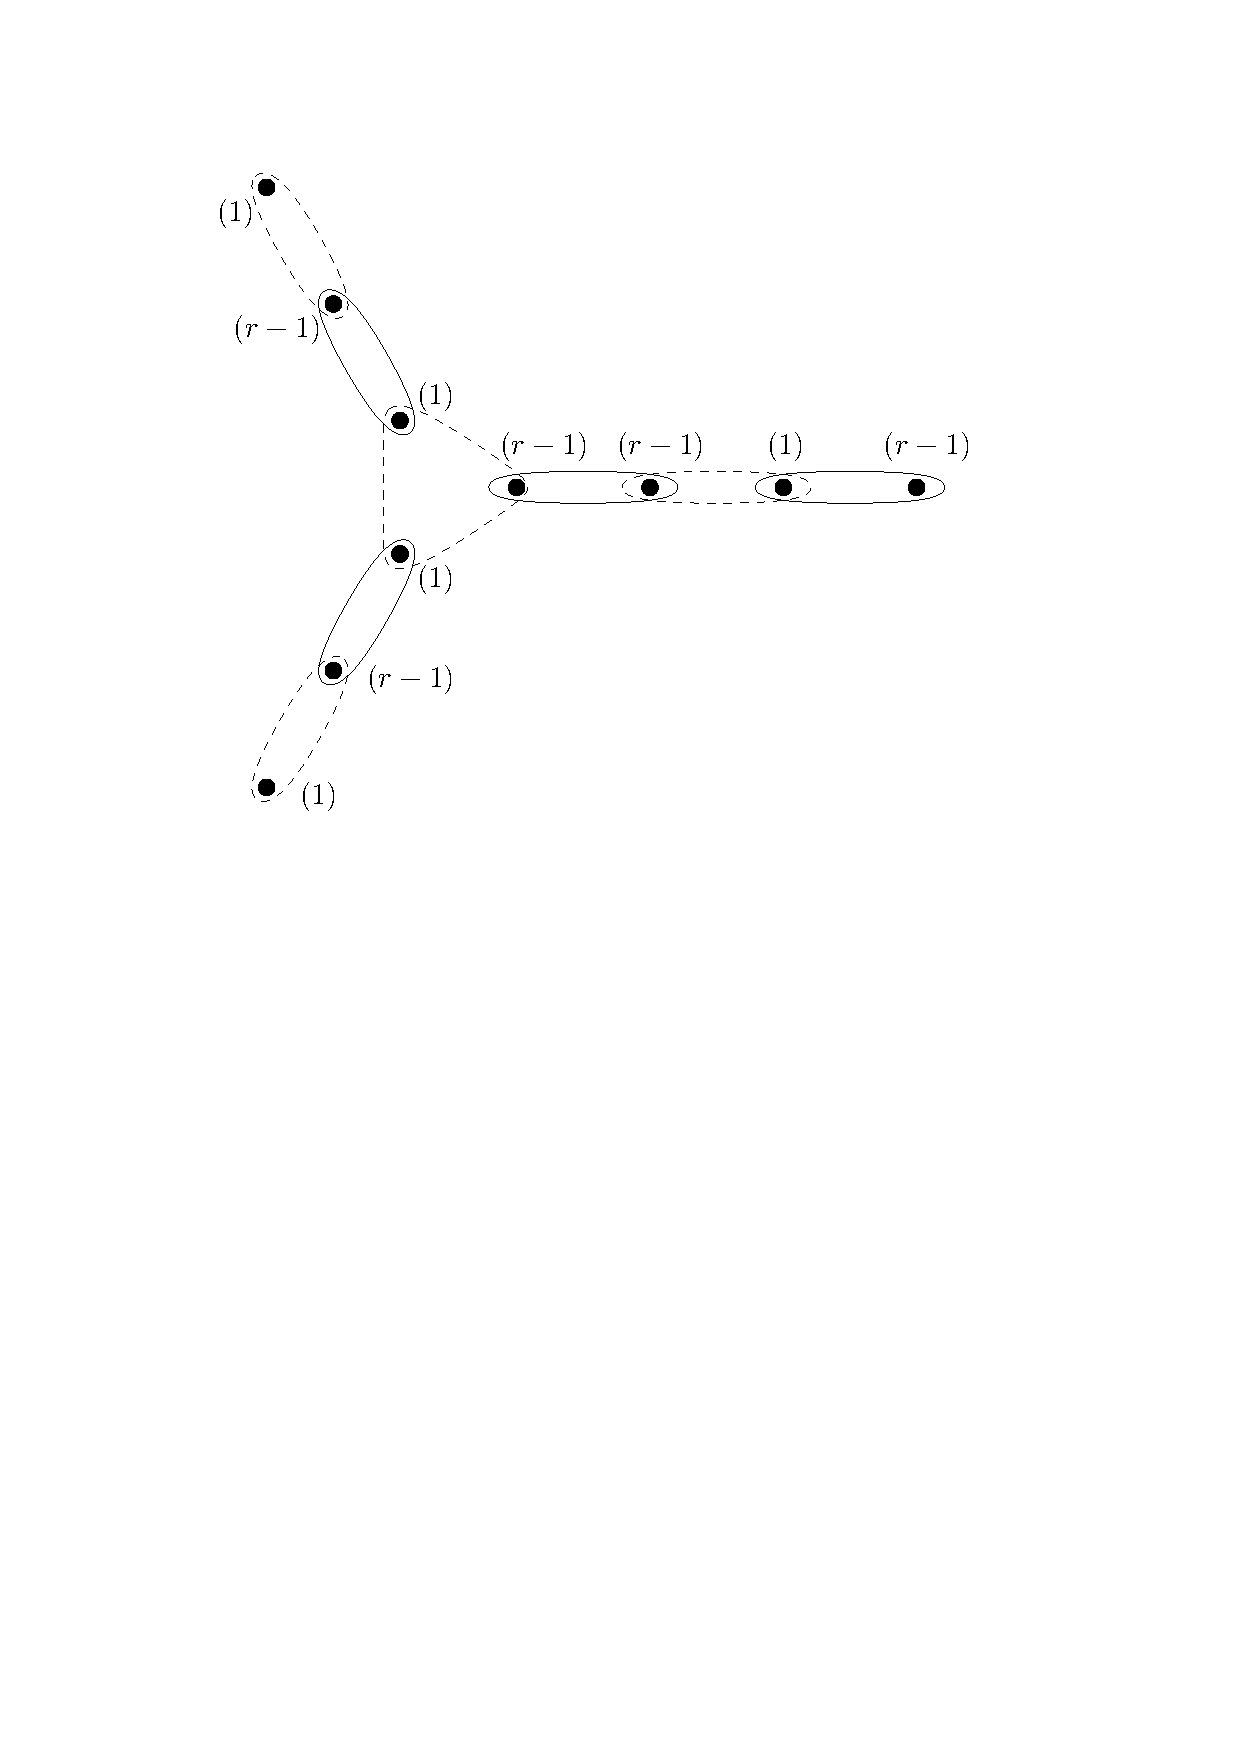
\includegraphics[width=.75\linewidth]{figs/nandgadget.pdf}
%\end{center}
%}



\frame{ \frametitle{Hardness}

How to correct at the splitter?
\pause \vskip .35cm

wlog, restrict ourselves to a certain configuration with two disks touching a third disk.
\pause \vskip .35cm

Then we compute optimal way for them to touch it $\rightarrow$ the 1.912 factor.

}


\frame{ \frametitle{Hardness}

\begin{center}
  \includegraphics<1>[page=1,width=.33\linewidth]{figs/correctanim.pdf}
\pause
  \includegraphics<2>[page=1,width=.5\linewidth]{figs/splitteranim.pdf}
%  \only<1>{\\Obs: both directions can't be bad---consider $\deg_L(v)$ v. $\deg_R(v)$.}
\pause
  \includegraphics<3>[page=2,width=.5\linewidth]{figs/splitteranim.pdf}
%  \only<2>{\\Obs: If $\deg_L(v) \le \deg_R(v)$, still true after moving left.}
\pause
  \includegraphics<4>[page=3,width=.5\linewidth]{figs/splitteranim.pdf}
\pause
  \includegraphics<5>[page=17,width=.5\linewidth]{figs/splitteranim.pdf}
\pause
  \includegraphics<6>[page=3,width=.5\linewidth]{figs/splitteranim.pdf}
%\pause
%  \includegraphics<6>[page=5,width=.5\linewidth]{figs/splitteranim.pdf}
\pause
  \includegraphics<7>[page=6,width=.5\linewidth]{figs/splitteranim.pdf}
\pause
  \includegraphics<8>[page=7,width=.5\linewidth]{figs/splitteranim.pdf}
\pause
  \includegraphics<9>[page=8,width=.5\linewidth]{figs/splitteranim.pdf}
\pause
  \includegraphics<10>[page=9,width=.5\linewidth]{figs/splitteranim.pdf}
\pause
  \includegraphics<11>[page=10,width=.5\linewidth]{figs/splitteranim.pdf}
\pause
  \includegraphics<12>[page=16,width=.5\linewidth]{figs/splitteranim.pdf}
\pause
  \includegraphics<13>[page=18,width=.5\linewidth]{figs/splitteranim.pdf}
\pause
  \includegraphics<14>[page=19,width=.5\linewidth]{figs/splitteranim.pdf}
\end{center}
}



\frame{ \frametitle{What about $r=3$?}


\begin{center}
  \includegraphics<1>[page=1,width=.33\linewidth]{figs/correctanim.pdf}
%  \only<1>{\\Obs: both directions can't be bad---consider $\deg_L(v)$ v. $\deg_R(v)$.}
\pause
  \includegraphics<2>[page=3,width=.33\linewidth]{figs/correctanim.pdf}
%  \only<2>{\\Obs: If $\deg_L(v) \le \deg_R(v)$, still true after moving left.}
\pause
  \includegraphics<3>[page=1,width=.33\linewidth]{figs/correctanim.pdf}
\pause
  \includegraphics<4>[page=10,width=.33\linewidth]{figs/correctanim.pdf}
\end{center}
}



\frame{ \frametitle{What about $r=2$?}

\begin{center}
  \includegraphics<1>[page=1,width=.33\linewidth]{figs/correctanim.pdf}
\pause
  \includegraphics<2>[page=11,width=.33\linewidth]{figs/correctanim.pdf}
\end{center}
}


%\frame{ \frametitle{What about pairwise distance cost?}
%
%\begin{center}
%  \includegraphics<1>[page=1,width=.33\linewidth]{figs/correctanim.pdf}
%\pause
%  \includegraphics<2>[page=12,width=.33\linewidth]{figs/correctanim.pdf}
%\end{center}
%}


%\frame{ \frametitle{Results}
%
%
%We obtain these hardness of approx factors:
%
%\pause \vskip .5cm
%
%%\begin{itemize}
%%\item for diameter as bounding disk:
%%\vskip .15cm\pause
%%\begin{itemize}
%%\item for $r=3$: $\sqrt{13}/2 \approx 1.802$
%%\item for $r \geq 4$: ${\sqrt{35}+\sqrt{3} \over 4} \approx 1.912$
%%\end{itemize}
%%
%%\pause \vskip .5cm
%%
%%\item for diameter as max pairwise dist:
%%\vskip .15cm\pause
%%\begin{itemize}
%%\item for $r=3,4$: $\sqrt{2+\sqrt{3}} \approx 1.931$
%%\item for $r \geq 5$: $2$
%%\end{itemize}
%%\end{itemize}
%
%
%\begin{table}[]
%\centering
%\small
%\begin{tabular}{@{}ccccc@{}}
%\toprule
%                                & $r=2$                     & $r=3$                                                           & $r=4$                                                             & $r\ge5$                                                           \\ \midrule
%\multicolumn{1}{c|}{disk diam} & \multicolumn{1}{|c|}{(in P)} & \multicolumn{1}{|c|}{$\sqrt{13}/2 \approx 1.802$}                & \multicolumn{1}{|c|}{${\sqrt{35}+\sqrt{3} \over 4} \approx 1.912$} & \multicolumn{1}{|c|}{same} \\ \midrule
%\multicolumn{1}{c|}{pair dist} & \multicolumn{1}{|c|}{(in P)} & \multicolumn{1}{|c|}{$\sqrt{2+\sqrt{3}} \approx 1.931$} & \multicolumn{1}{|c|}{same}   & \multicolumn{1}{|c|}{$2$}                                             \\ \bottomrule
%\end{tabular}
%\end{table}
%
%}


%\frame{ \frametitle{NP-Complete?}
%
%NP-hard, but in NP?
%\vskip .25cm
%
%Not clear: high-precision coordinates...
%\vskip .25cm
%\pause
%Recall hard game instance:
%%\pause
%%  \includegraphics[width=.35\linewidth]{plangame3}
%\pause
%Conjecture: can restrict drawings WLOGto convex position (e.g., nodes on a circle).
%\vskip .25cm
%
%Convex conjecture $\rightarrow$ clearly MRCN is in NP. (Then drawing = permutation.)
%\vskip .25cm
%}

\section{Algorithms}
\subsection{}

\frame{ \frametitle{Algorithms}

\pause
Nope!
}




\section{Conclusion}
\subsection{}


\frame{ \frametitle{Conclusion}

So: restricting from metric to Euclidean plane, achieved hardness of approx approaching 2:
\vskip .25cm\pause 

$\sqrt{3} \approx 1.73$ \pause $~\rightarrow~$ \pause $1+{\sqrt{3} \over 2} \approx 1.866$ \pause $~\rightarrow~$ \pause ${\sqrt{3}+\sqrt{35} \over 4} \approx 1.912$ \pause $~\not \rightarrow~ 2$
\vskip .25cm\pause 

But gap remains, and no improvement in positive results
\vskip .35cm\pause

Complimentary optimization goal: maximize $r$, given hard constraint on diameter $d$ \pause
\begin{itemize}
\item hardness proof for $r=3$ case $\rightarrow$ hard to approx for $c_r<{2 \over 3}$
\item {\em no known approx alg}
\end{itemize}
\vskip .35cm\pause


$\rightarrow$ bicriteria problem for $(d,r)$
\pause
\begin{itemize}
\item Original 2-approx here: $(2,1)$
\pause

\item Alt goal: $(1,c_r)$ for some $c_r \in (0,1)$ \pause (as yet unsuccessful)
\vskip .35cm\pause

\item More modest goal: $(c_d,c_r)$ for some $c_r \in (0,1)$ and some $c_d < 2$ \pause (also unsuccessful!!)
\end{itemize}
}

\frame{ \frametitle{Conclusion}


\begin{table}[]
\centering
\small
\begin{tabular}{@{}ccccc@{}}
\toprule
                                & $r=2$                     & $r=3$                                                           & $r=4$                                                             & $r\ge5$                                                           \\ \midrule
\multicolumn{1}{c|}{disk diam} & \multicolumn{1}{|c|}{(in P)} & \multicolumn{1}{|c|}{$\sqrt{13}/2 \approx 1.802$}                & \multicolumn{1}{|c|}{${\sqrt{35}+\sqrt{3} \over 4} \approx 1.912$} & \multicolumn{1}{|c|}{same} \\ \midrule
\multicolumn{1}{c|}{pair dist} & \multicolumn{1}{|c|}{(in P)} & \multicolumn{1}{|c|}{$\sqrt{2+\sqrt{3}} \approx 1.931$} & \multicolumn{1}{|c|}{same}   & \multicolumn{1}{|c|}{$2$}                                             \\ \bottomrule
\end{tabular}
\end{table}

\vskip 1.5cm
\begin{center}
Thanks!

mpjohnson@gmail.com
\end{center}
}






\end{document}